%% Computer Methods and Programs in Biomedicine — revised manuscript
%% (CMPB-D-26-05530). Revisions are shown in red; the superscript tag
%% before each change gives the reviewer comment it answers
%% (R1.x = Reviewer 1, R2.x = Reviewer 2, AC = author correction).
%% Template: elsarticle 5p (two-column, Times)
\documentclass[5p,times,twocolumn]{elsarticle}

\usepackage{amsmath}
\usepackage{amssymb}
\usepackage{amsfonts}
\usepackage{graphicx}
\usepackage{booktabs}
\usepackage{multirow}
\usepackage{makecell}
\usepackage{array}
\usepackage{subcaption}
\usepackage[ruled,linesnumbered]{algorithm2e}
\usepackage[table]{xcolor}
\usepackage{balance}
\usepackage{hyperref}

%% ---- revision highlighting ----------------------------------------
%% \rtag{R1.2}            superscript comment tag (red, bold)
%% \rev{R1.2}{text}       tagged inline red text
%% \begin{revblock}{R1.2} ... \end{revblock}   tagged red block
%%                        (paragraphs, equations, lists)
\newcommand{\rtag}[1]{\textsuperscript{\textcolor{red}{\textbf{#1}}}}
\newcommand{\rev}[2]{\rtag{#1}\textcolor{red}{#2}}
\newenvironment{revblock}[1]{\par\color{red}\rtag{#1}\ignorespaces}{\par}
%% \lang{text}  language correction (R1.15, R2.25): red, untagged
\newcommand{\lang}[1]{\textcolor{red}{#1}}

\journal{Computer Methods and Programs in Biomedicine}

\begin{document}

\begin{frontmatter}

  \title{Proteomics-Integrated Digital Twin State Space for Dopaminergic Stem Cell Differentiation}

  % \author[kit]{Victor Ikenna Kanu}
  % \author[lu]{Willaims Paul Nwadiugwu}
  % \author[kit]{Dong-Seong Kim\corref{cor}}
  % \cortext[cor]{Corresponding author}
  % \affiliation[kdu]{organization={Smart Computing Department, Kyungdong University, Global Campus}, country={South Korea}}
  % \affiliation[kit]{organization={Department of IT Convergence Engineering,
  %   Kumoh National Institute of Technology}, city={Gumi},
  %   country={South Korea}}

  \begin{abstract}
    \color{red}
    \rtag{R1.1,R2.1,R1.14}Transcriptomic digital twins of stem cell
    differentiation omit the protein layer, where drug targets act.
    This study constructs and validates a proteomics-integrated
    state representation for dopaminergic differentiation of induced
    pluripotent stem cells (iPSC-DA). A published two-dimensional
    transcriptomic state, comprising a pluripotency score $P_{t}$
    and a dopaminergic score $D_{t}$ derived from 161,584 single
    cells at stages D11, D30, and D52, is extended to
    $\mathbf{s}_{t} = [P_{t}, D_{t}, Pr_{t}]$ by adding a proteomic
    score $Pr_{t}$ computed from the abundance of TH, DDC, ALDH1A1,
    and COMT in label-free proteomics from a separate iPSC-DA study.
    Linear, Random Forest, and Transformer models are evaluated on
    two distinct questions, stage separability and trajectory
    prediction, over 20 seeds, with permutation nulls, a
    $Pr_{t}$-only baseline, and leave-one-replicate-out analysis,
    while SHA-256 fingerprints of all inputs are recorded on the
    PureChain blockchain for verifiable provenance.
    \rtag{R1.8,R2.12}The 3D state separates the three stages
    perfectly (macro F1 $= 1.000$ for all models), but $Pr_{t}$
    alone does the same, so this reflects separability along the
    proteomic axis rather than model superiority.
    \rtag{R1.4,R1.9,R2.13}For trajectory prediction, the 3D state
    lowers mean absolute error by 28--31\% (95\% bootstrap
    confidence intervals within $-25.6\%$ to $-31.9\%$; paired
    Wilcoxon $p < 10^{-3}$), a gain that comes entirely from the
    added, well-forecastable $Pr_{t}$ dimension, while errors on
    $P_{t}$ and $D_{t}$ are unchanged.
    \rtag{R1.5,R2.8,R2.20}Measured proteomics therefore adds stage
    information that transcriptomics lacks without degrading
    transcriptomic forecasts. Because the proteomic axis rests on
    only 3/2/2 control replicates from a separate study,
    confirmation on paired, larger, and independent datasets is
    needed before the framework is applied to perturbation-aware
    drug screening in Parkinson's disease.
  \end{abstract}

  \begin{keyword}
    Digital twin \sep
    Dopaminergic differentiation \sep
    Multi-omics state space \sep
    Proteomics integration \sep
    Distributed ledger provenance
  \end{keyword}

\end{frontmatter}

\section{Introduction}

Parkinson's disease (PD) is one of the fastest-growing
neurological disorders worldwide, characterised by the
progressive and irreversible loss of dopaminergic (DA)
neurons in the substantia nigra pars compacta,
depleting striatal dopamine and producing the hallmark
motor symptoms of bradykinesia, rigidity, and resting
tremor~\cite{jang2020current}.
Although pharmacological dopamine replacement therapies
provide symptomatic relief in the early stages of
disease, their efficacy declines over time while
side-effect burden accumulates, leaving patients without
a disease-modifying intervention~\cite{barker2024history}.
\lang{Attention has therefore turned to}
iPSC-derived DA (iPSC-DA) neurons as a patient-matched
cellular substrate for both transplantation therapy
and in vitro drug screening~\cite{oz2023neural}.
Yet \lang{predicting} iPSC-DA maturation
across discrete differentiation stages\rev{AC}{ ---
  early floor-plate progenitor (D11), transitional (D30),
  and mature dopaminergic (D52) ---} remains an open computational challenge,
limiting the utility of these models in drug
development pipelines.

Computational digital twins (DTs) --- virtual replicas
that mirror and forecast biological system state ---
have emerged as a principled framework for this
challenge~\cite{masison2021modular}.
Recent DT approaches for stem cell differentiation
have relied exclusively on \lang{transcriptomic state
  representations}, capturing gene expression dynamics
but remaining blind to the protein layer where \lang{drug
  candidates} must ultimately exert their effect.
This is a significant limitation. mRNA and protein abundance correlate weakly across tissues~\cite{kosti2016cross}. The most drug-relevant molecular behaviours, such as enzyme activity, receptor occupancy, and signalling pathway states, are protein-level phenomena \lang{for which transcript levels are not a reliable proxy}.
For dopaminergic differentiation specifically,
tyrosine hydroxylase (TH) protein abundance directly
governs the rate of dopamine synthesis, making protein
measurement indispensable for any DT intended to
guide drug screening decisions.

Beyond the biological incompleteness of transcriptomic DTs, reproducibility challenges compound the problem for multi-source computational pipelines.
Assembling scRNA-seq data from one laboratory with proteomics from another introduces provenance risks absent from single-source workflows. Dataset versions change silently, preprocessing decisions are underreported, and no standard mechanism exists for independent researchers or regulatory reviewers to verify that published results were derived from the claimed data~\cite{johns2023data}.
Distributed ledger technology (DLT), with its immutable audit trail and tamper-proof data fingerprinting, has been proposed as a principled solution to this problem~\cite{kuo2017blockchain}. However, its application to multi-omics DT pipelines has not been demonstrated.

Taken together, these gaps \lang{point to an unmet need}: a digital twin for iPSC-DA
differentiation that integrates protein-level state
information, is validated against rigorous statistical
nulls, and is underpinned by verifiable DLT-secured
data provenance.
This study directly addresses that need by extending
a published two-dimensional transcriptomic state
space $(P, D)$ to a proteomics-integrated
three-dimensional state
$\mathbf{s}_{t} = [P_{t}, D_{t}, Pr_{t}]$,
benchmarked across multiple model families with
permutation-validated signal confirmation and
supported by a deployed DLT provenance layer.

\begin{revblock}{R1.1,R2.1,R2.21}
The primary objective of this study is
  the construction and validation of a proteomics-integrated
  state representation for iPSC-DA differentiation. Two
  questions are asked of this representation, and they are
  kept separate throughout the paper:
  \textit{(O1) stage separability} --- does the added
  proteomic axis distinguish the three differentiation stages
  that the transcriptomic axes confuse? (Task~A); and
  \textit{(O2) trajectory prediction} --- does the 3D state
  improve forecasting of the late-stage state from earlier
  states, and on which axes? (Task~B).
  O1 is a diagnostic of the representation rather than a
  predictive goal in itself; O2 is the forecasting question
  for which a digital twin is ultimately intended.
  The blockchain provenance layer is a secondary, supporting
  contribution that makes the multi-source pipeline
  verifiable; it does not affect any modelling result.
  In order of importance, the four contributions of this
  work are:
\end{revblock}

\begin{enumerate}
  \item \textbf{A proteomics-integrated 3D state space}
  for a multi-omics DT,
  $\mathbf{s}_{t} = [P_{t}, D_{t}, Pr_{t}]$,
  constructed by integrating transcriptomic and
  label-free proteomic marker sets under a principled
  curation protocol, extending transcriptomic-only DT
  baselines to the protein layer where drug targets
  reside.
  \item \textbf{A multi-seed, multi-control evaluation
    framework} benchmarking the 3D state against the 2D
  baseline across three model families on stage
  separability and trajectory prediction over 20 seeds,
  combining permutation nulls, a leave-one-replicate-out
  probe, and a single-feature baseline with paired
  significance testing to confirm \lang{that} the gains reflect
  genuine proteomic-stage signal rather than added model
  capacity.
  \item \textbf{A cross-modal orthogonality and
    error-decomposition analysis} confirming that the
  \rev{AC}{assembled proteomic dimension introduces no spurious
    coupling with} the transcriptomic axes and that the
  trajectory-prediction gain reflects a forecastable
  added dimension rather than altered forecasts of the
  original axes.
  \item \textbf{A deployable DLT provenance layer} via a
  \texttt{MultiOmicsProvenance} smart contract on the
  PureChain mainnet that records immutable SHA-256
  fingerprints of all raw inputs and processed outputs
  at every pipeline stage, providing independent
  reproducibility verification for all results reported.
\end{enumerate}

%%────────────────────────────────────────────────────────────────────
\section{Related Works}

\subsection{\textbf{Digital Twins for Biological Systems}}

Digital twin technology, originally developed for
engineering systems, has been progressively adapted
to biomedical applications, as the availability of
high-dimensional molecular data has
grown~\cite{masison2021modular}.
\rev{R1.16}{In engineering, state-space digital twins combined
  with predictive control already support real-time stability
  monitoring~\cite{pandey2026statespace}; the present work
  applies the same state-space view of a digital twin to a
  biological differentiation process.}
In the clinical domain, DT frameworks have been
applied to patient-specific disease trajectory
modelling, treatment response forecasting, and
personalised medicine, demonstrating the viability
of virtual replicas as decision-support
tools~\cite{hansen2024transcriptomics}.
At the cellular level, authors~\cite{li2022dynamic}
proposed a dynamic single-cell DT framework
that leverages scRNA-seq data to prioritise
drug targets by simulating gene regulatory
network perturbations, representing the most
direct prior attempt to connect DT modelling
with drug discovery in a single-cell context.
More recently, DT architectures have been
integrated with federated learning and
informatics infrastructure for intelligent
biomedical diagnostics~\cite{qu2023dtqfl}.
Despite this progress, existing biological DTs
share a critical limitation: their state
representations are constructed exclusively from
transcriptomic data, with no existing framework
incorporating measured protein-level information
into the DT state space.

\subsection{\textbf{Transcriptomic Modelling of Stem Cell
    Differentiation}}

Single-cell RNA sequencing has transformed the
study of stem cell differentiation by enabling
population-scale characterisation of stage-specific
gene expression \lang{programmes}~\cite{jerber2021population}.
On the computational side, several approaches have
been developed to extract temporal dynamics from
scRNA-seq snapshots.
Authors~\cite{erbe2023transcriptomic} applied neural ordinary
differential equations to continuous-time
transcriptomic forecasting, demonstrating that
data-driven models can capture differentiation
trajectories from metabolic-labelling time courses.
Authors~\cite{chen2023transformer} introduced
a Transformer architecture for interpretable
cell-type annotation, establishing the viability
of attention-based models for single-cell
classification tasks.
Authors~\cite{farrell2023inferring} combined
variational autoencoders with structured neural
ODEs to infer RNA velocity and lineage-aware
trajectories, while authors~\cite{jiang2024physics}
incorporated physical constraints into neural
stochastic differential equations for learning
cellular dynamics from scRNA-seq time series.
These methods have significantly advanced
trajectory inference and velocity estimation,
yet they share two limitations relative to the
present work: they target \lang{continuous trajectory
  inference rather than discrete stage-to-stage
  forecasting}, and they operate exclusively within
the transcriptomic modality.

\subsection{\textbf{Multi-Omics Integration and the
    Protein-Level Gap}}

The discordance between mRNA and protein abundance
is a well-documented phenomenon across tissue types,
with Spearman correlations typically ranging from
0.36 to 0.50~\cite{kosti2016cross}, arising from
differences in translation efficiency, protein
half-lives, and post-transcriptional
regulation.
In the context of drug development, this discordance
has concrete consequences: \rev{AC}{Authors~\cite{tasaki2022inferring}
  showed that protein-level changes in diseased tissue are
  only partly predictable from mRNA, a limitation that
  applies to any computational framework relying on mRNA
  as a proxy for protein activity}.
In the iPSC context specifically, proteomic
measurements reveal population-scale variation
linked to disease-relevant \lang{genome-wide association study} (GWAS) loci that is
undetectable at the mRNA level~\cite{mirauta2020population}.
At the iPSC-DA differentiation level, Novak et al.\
\cite{novak2022single} provided the first paired
transcriptomic and proteomic profiling of iPSC-DA
cultures, identifying protein-level markers of
dopaminergic maturation and PINK1-linked
Parkinson's pathology.
The depth of publicly available iPSC-DA proteomics
was subsequently extended by Cavarischia-Rega et al.\
\cite{cavarischia2024proteome}, who profiled 9,409
protein groups in iPSC-derived dopaminergic neurons,
confirming that canonical dopaminergic transcription
factors remain below the detection limit of
standard whole-cell-lysate workflows.
Collectively, this body of work \lang{establishes} both the
measurability and the biological \lang{relevance} of
protein-level information in iPSC-DA systems,
yet no prior study has incorporated proteomics
into a DT state space for differentiation
forecasting.

\subsection{\textbf{Distributed Ledger Technology for
    Biomedical Reproducibility}}
\label{sec:rw_dlt}

The reproducibility crisis in computational
biomedicine is \lang{well documented}: a scoping review
of 44 provenance studies found that most biomedical
pipelines record only source-level provenance
without capturing the processing steps that
transform raw data into results~\cite{johns2023data}.
Authors~\cite{kuo2017blockchain} established the
foundational case for DLT in biomedical informatics,
identifying immutable audit trails and data
provenance as the primary benefits of
blockchain-based approaches over traditional
distributed database systems.
Subsequent work has extended DLT applications
to clinical trial data integrity, electronic health
record sharing, and federated biomedical data
governance, with systematic reviews confirming
the maturity of the approach for institutional
deployments~\cite{lacson2024biomedical}.
In the multi-omics domain, the convergence of DLT
with digital twins and multi-omics platforms has
been identified as a transformative direction for
personalised medicine~\cite{mohr2024navigating}.
However, no existing multi-omics computational
pipeline has deployed a DLT provenance layer
that records both raw data fingerprints and
processing-step version anchors in a single,
independently queryable on-chain record.

\subsection{\textbf{Challenges}}

Despite these \lang{advances}, several challenges
remain in building effective multi-omics DTs
for iPSC-DA differentiation.
Transcriptomic and proteomic datasets are rarely
time-matched across protocols, and the absence
of standardised preprocessing introduces
modality-specific batch effects that confound
multi-omics state space
construction~\cite{mohr2024navigating}.
Furthermore, standard whole-cell-lysate proteomics
systematically misses nuclear transcription factors
and membrane channels central to DA-neuron identity,
a constraint confirmed \rev{AC}{in the deepest publicly
  available iPSC-DA
  proteome}~\cite{cavarischia2024proteome}.
At the validation level, few existing DT studies
employ permutation-based null experiments to
rigorously distinguish genuine cross-modal signal
from artefacts of added model
capacity~\cite{mohr2024navigating}, leaving the
biological interpretability of reported
improvements unresolved.
Finally, while DLT has demonstrated value for
biomedical data governance~\cite{lacson2024biomedical},
existing implementations address access control
and sharing, but none \lang{provides a deployable}
provenance layer that records both raw data
fingerprints and pipeline-version anchors across
heterogeneous omics ingestion steps.
The present work addresses each of these challenges
within a unified, reproducible framework for
\lang{constructing DTs of iPSC-DA differentiation}.
%% ============================================================
%%  LIST OF ABBREVIATIONS
%%  Place after the abstract and before the Introduction,
%%  or after keywords depending on journal template.
%%  elsarticle: place before \section{Introduction}
%% ============================================================

\begin{figure*}[!htbp]
  \centering
  %% R1.6: printed width increased from 0.55 to 0.65\linewidth so the
  %% pipeline labels are legible.
  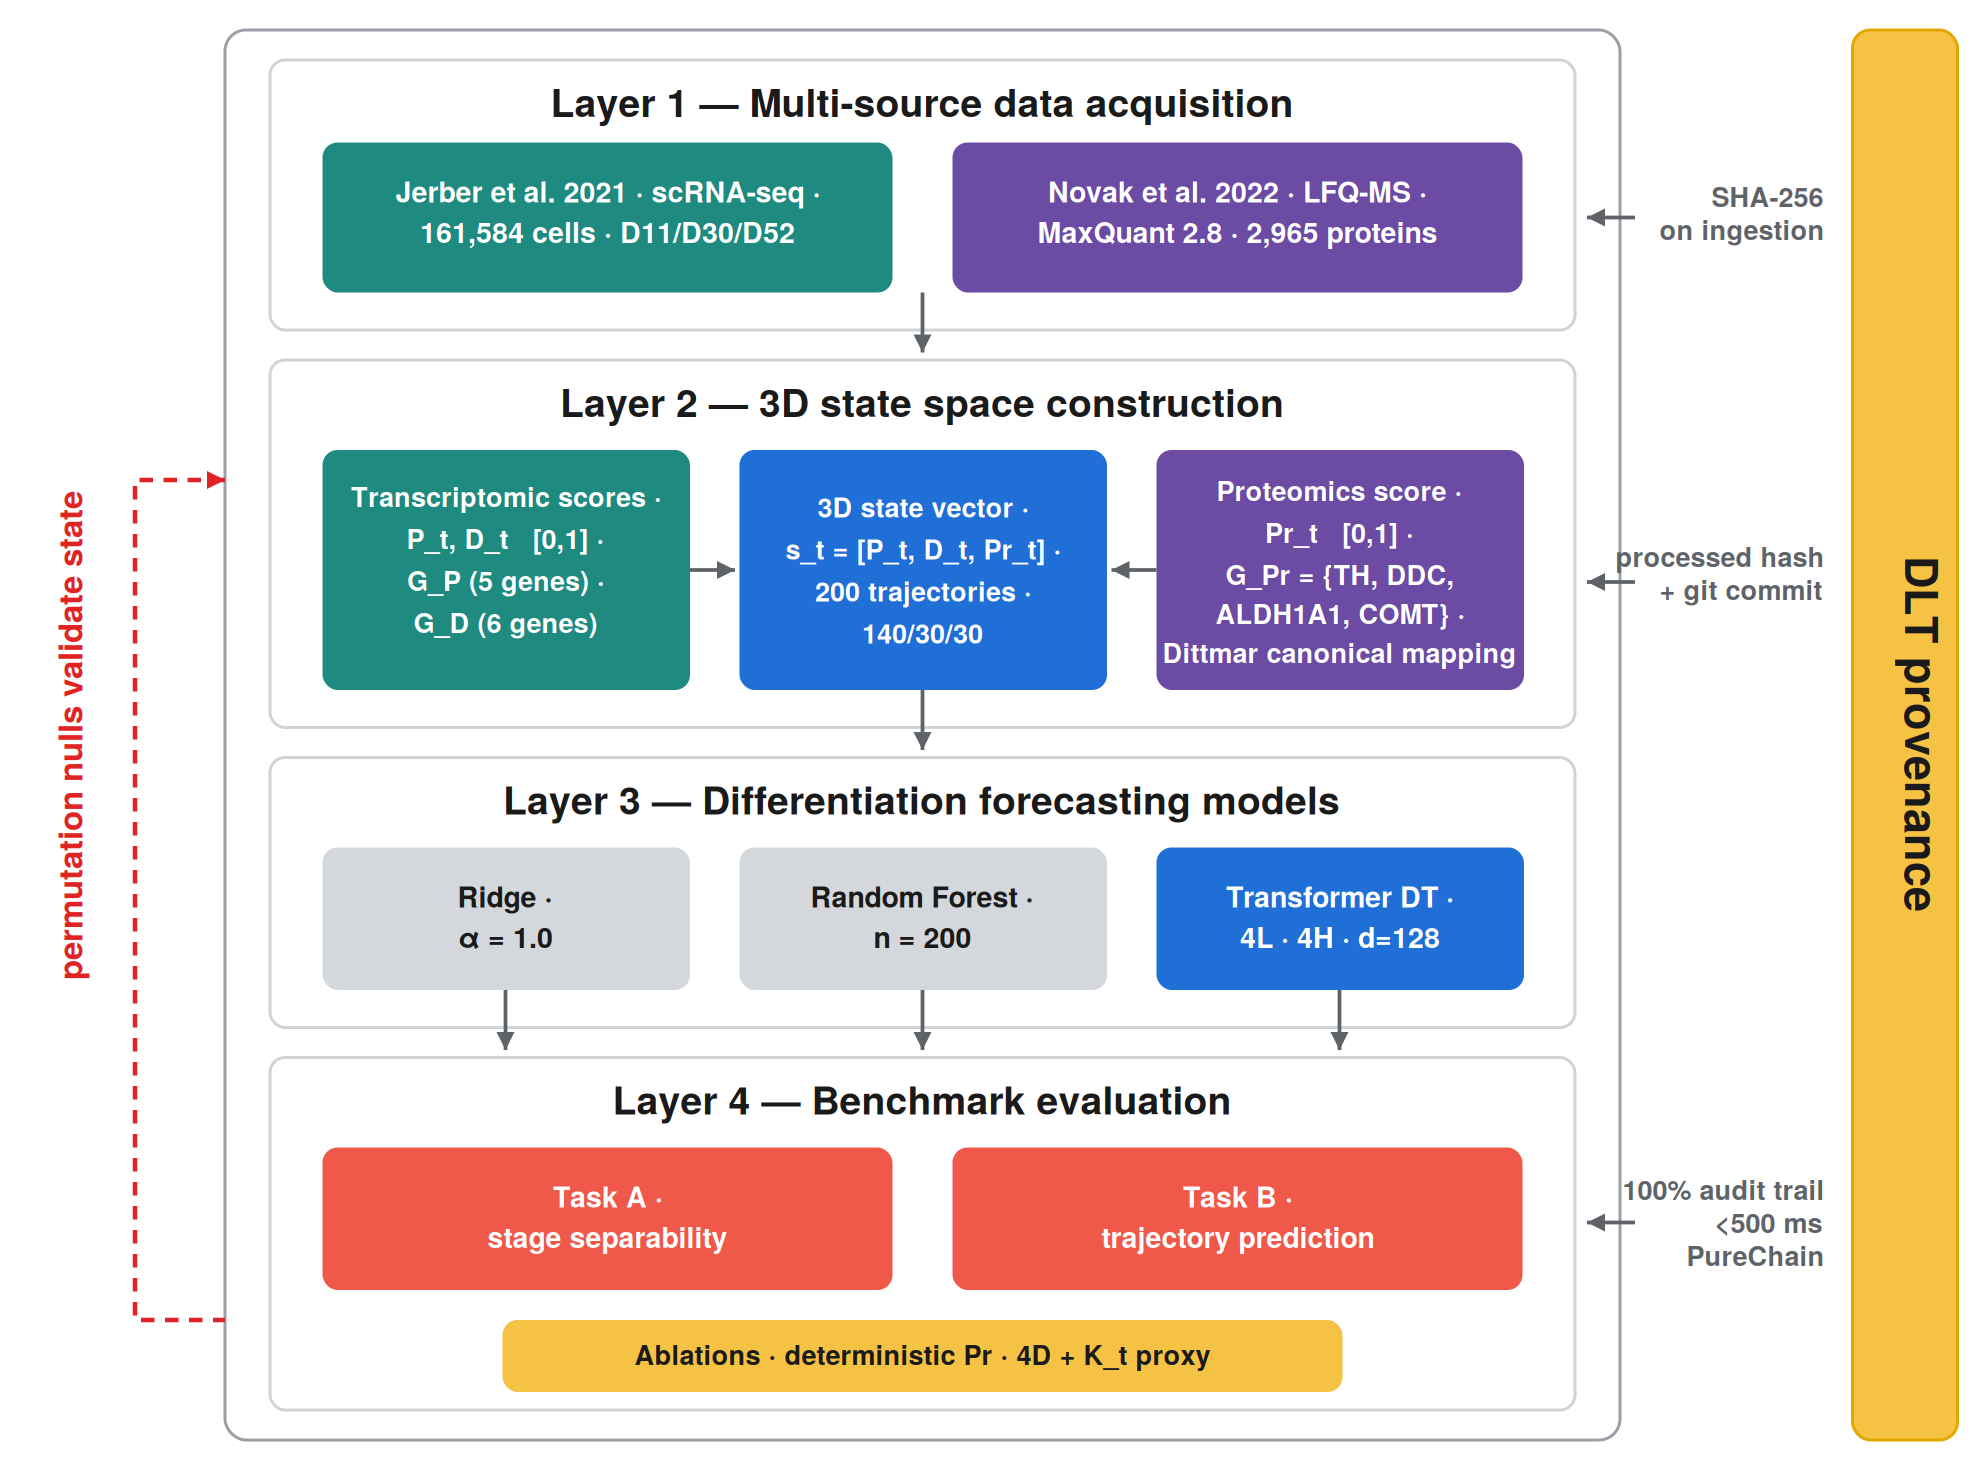
\includegraphics[width=0.70\linewidth]{images/fig1_pipeline.png}
  \caption{Proteomics-integrated digital twin pipeline for
    dopaminergic stem cell differentiation.
    Transcriptomic scRNA-seq~\cite{jerber2021population} and
    re-processed label-free
    proteomics~\cite{novak2022single} are harmonised
    into a 3D state vector
    $\mathbf{s}_{t} = [P_{t}, D_{t}, Pr_{t}] \in [0,1]^{3}$
    ($N = 200$ trajectories, split 140/30/30) and benchmarked
    across \rev{R1.6,AC}{a linear model (logistic regression
      for Task~A, Ridge regression for Task~B)}, Random Forest,
    and Transformer DT models
    on stage separability (Task~A) and trajectory prediction
    (Task~B).
    \rev{R1.6}{The figure is printed at a larger size in this
      revision for legibility.}
    The amber bar denotes the PureChain blockchain provenance
    layer: SHA-256 fingerprints are registered at ingestion
    and after processing.
    The red dashed arrow indicates that permutation, leave-one-replicate-out,
    and single-feature analyses validate the state space rather
    than model capacity.}
  \label{fig:pipeline}
\end{figure*}

\begin{table}[!htbp]
  \centering
  \scalebox{0.75}{
    \begin{tabular}{p{2.7cm} p{6.2cm}}
      \toprule
      \textbf{Abbreviation} & \textbf{Definition} \\
      \midrule
      \multicolumn{2}{l}{\textit{Biology}} \\
      \midrule
      scRNA-seq   & Single-cell RNA sequencing \\
      iPSC        & Induced pluripotent stem cell \\
      iPSC-DA     & iPSC-derived dopaminergic neuron \\
      DA          & Dopaminergic \\
      PD          & Parkinson's disease \\
      TH          & Tyrosine hydroxylase \\
      DDC         & DOPA decarboxylase \\
      COMT        & Catechol-O-methyltransferase \\
      ALDH1A1     & Aldehyde dehydrogenase 1 family member A1 \\
      NR4A2       & Nuclear receptor subfamily 4 group A member 2 (NURR1) \\
      LMX1B       & LIM homeobox transcription factor 1 beta \\
      KCNJ6       & Potassium inwardly rectifying channel subfamily J member 6 (GIRK2) \\
      FOXA2       & Forkhead box protein A2 \\
      TF          & Transcription factor \\
      LFQ         & Label-free quantification \\
      MS          & Mass spectrometry \\
      PSM         & Peptide-spectrum match \\
      FDR         & False discovery rate \\
      MAPK        & Mitogen-activated protein kinase \\
      PI3K        & Phosphoinositide 3-kinase \\
      AKT         & Protein kinase B \\
      \midrule
      \multicolumn{2}{l}{\textit{Computational and modelling}} \\
      \midrule
      DT          & Digital twin \\
      2D          & Two-dimensional \\
      3D          & Three-dimensional \\
      4D          & Four-dimensional \\
      MAE         & Mean absolute error \\
      F1          & F1 score (harmonic mean of precision and recall) \\
      LORO        & Leave-one-replicate-out \\
      RF          & Random Forest \\
      LR          & Logistic Regression \\
      ODE         & Ordinary differential equation \\
      $P_t$       & Pluripotency score at timepoint $t$ \\
      $D_t$       & Dopaminergic differentiation score at timepoint $t$ \\
      $Pr_t$      & Proteomics score at timepoint $t$ \\
      $K_t$       & Transcript-derived kinase activity score at timepoint $t$ \\
      $\mathcal{G}_P$  & Pluripotency marker gene set \\
      $\mathcal{G}_D$  & Dopaminergic differentiation marker gene set \\
      $\mathcal{G}_{Pr}$ & Proteomics marker protein set \\
      \midrule
      \multicolumn{2}{l}{\textit{IT and infrastructure}} \\
      \midrule
      DLT         & Distributed ledger technology \\
      EVM         & Ethereum Virtual Machine \\
      SHA-256     & Secure Hash Algorithm 256-bit \\
      RPC         & Remote procedure call \\
      ENA         & European Nucleotide Archive \\
      PRIDE       & PRoteomics IDEntifications database \\
      \midrule
      \multicolumn{2}{l}{\textit{Timepoints}} \\
      \midrule
      D11         & Differentiation day 11 (\rev{AC}{floor-plate progenitor stage}) \\
      D25         & Differentiation day 25 (Novak et al. protocol) \\
      D30         & Differentiation day 30 (transitional stage) \\
      D40         & Differentiation day 40 (Novak et al. protocol) \\
      D52         & Differentiation day 52 (mature DA neuron stage) \\
      \bottomrule
    \end{tabular}}
\end{table}

\section{Methodology}

% -----------------------------------------------------------------
\subsection{\textbf{Transcriptomic DT baseline}}
\label{sec:baseline}

The 2D transcriptomic state space used as
the baseline in this study was established for dopaminergic
stem cell differentiation forecasting using scRNA-seq data~\cite{kanu2026transformer}.
Each cell at timepoint $t$ is represented by two biologically
grounded scores: a pluripotency score $P_{t}$, derived from
the mean log-normalised expression of five stem-cell identity
genes
$\mathcal{G}_{P} = \{\text{POU5F1, NANOG, SOX2, UTF1, TDGF1}\}$,
and a dopaminergic differentiation score $D_{t}$, derived
from six dopamine-neuron marker genes
$\mathcal{G}_{D} = \{\text{TH, DDC, SLC6A3, DRD2, LMX1A, FOXA2}\}$.
\rev{R2.6,AC}{Both scores are scaled to $[0,1]$ with fixed
  min-max bounds taken over all 161,584 untreated cells
  ($P \in [0, 1.602]$, $D \in [0, 1.684]$ before scaling), as in
  the published baseline (Section~\ref{sec:state} discusses why
  this does not leak label information).}
\lang{The baseline model is a} Transformer encoder (4 layers, 4 attention heads,
$d_{\text{model}} = 128$, feedforward dimension 512,
dropout 0.1)\lang{,} trained on $N = 200$ sampled trajectories
split 140/30/30 (seed 42).
The present work extends this 2D baseline by integrating
a proteomics dimension; the full pipeline is illustrated
in Figure~\ref{fig:pipeline}.

% -----------------------------------------------------------------
\subsection{\textbf{Datasets}}
\label{sec:datasets}

The pipeline (Figure~\ref{fig:pipeline}, Layer~1) ingests two
independent public datasets: a transcriptomic scRNA-seq
resource and a proteomic mass-spectrometry resource.
Both sources are registered on the PureChain blockchain at
the point of ingestion, as described in
Section~\ref{sec:dlt}.

\subsubsection{Transcriptomics}
Single-cell RNA sequencing (scRNA-seq) profiles were obtained
from the dopaminergic differentiation dataset of
Jerber et al.~\cite{jerber2021population}, accessed via the
European Nucleotide Archive (ENA accession \texttt{PRJEB38269})
and Zenodo (\texttt{doi:10.5281/zenodo.4333872}).
After filtering to untreated samples (\texttt{treatment = NONE}),
161,584 quality-controlled cells were retained across three
ground-truth experimental timepoints: D11 ($n = 50{,}661$),
D30 ($n = 50{,}169$), and D52 ($n = 60{,}754$).
Raw counts were normalised using
\texttt{scanpy.pp.normalize\_total} (target sum $= 10^{4}$)
followed by \lang{a $\log(1+x)$} transformation.
The marker gene sets $\mathcal{G}_{P}$ and $\mathcal{G}_{D}$
defined in Section~\ref{sec:baseline} were used without
modification.

\subsubsection{Proteomics re-processing}
Proteomic data were sourced from Novak et al.~\cite{novak2022single}
(PRIDE accession \texttt{PXD028283}), comprising eight raw
Orbitrap mass-spectrometry files (\texttt{Skupin11--Skupin18},
$\approx 9$\,GB) acquired from iPSC-derived dopaminergic
(iPSC-DA) cultures at differentiation stages D25 and D40.
The public PRIDE deposit provides a curated 127-protein subset
of differentially abundant proteins between CTRL and PINK1
conditions; none of the canonical dopaminergic markers required
for $\mathcal{G}_{Pr}$ \lang{is} retained in this curation because
they are not differentially abundant between conditions.
Raw spectra were therefore re-processed locally with
MaxQuant 2.8.0.0~\cite{cox2008maxquant}, using the UniProt
human reviewed Swiss-Prot database (20,431 sequences),
trypsin/P digestion (maximum two missed cleavages),
carbamidomethylation as a fixed modification, oxidation and
acetylation as variable modifications, a 1\% false discovery
rate at the PSM and protein level, label-free quantification
(LFQ, minimum ratio count $= 2$), and match-between-runs
enabled.
This \lang{re-processing} recovered 2,965 protein groups --- 23$\times$ the
public curation --- including the canonical DA-pathway
proteins TH, DDC, ALDH1A1, and COMT.

\begin{revblock}{R2.4}
  \textbf{Proteomic data used for the reported results.}
  The local re-processing above covers only the eight
  deposited D25/D40 raw files and is used solely for the
  robustness check at the end of
  Section~\ref{sec:matching}.
  All $Pr$ values in the Results are computed from the
  canonical MaxQuant \texttt{proteinGroups} table of the same
  study, provided by the original
  authors~\cite{novak2022single}, which additionally contains
  the iPSC samples and carries the biological sample label of
  every column.
  It was processed as follows.
  \textit{(i) Filtering:} protein groups flagged as reverse
  (decoy) hits, potential contaminants, or identified only by
  a modification site were removed (3,669 $\to$ 3,577 groups).
  \textit{(ii) Gene mapping:} groups listing several gene
  names were split into one row per gene, and LFQ intensities
  of the same gene appearing in more than one group were
  summed on the linear scale.
  \textit{(iii) Sample selection:} only the seven healthy
  control (CTRL) columns were used
  (Section~\ref{sec:matching}); the columns of the PINK1 and
  other non-control lines were excluded so that disease effects
  cannot enter the stage signal.
  \textit{(iv) Missing values:} no imputation was applied.
  A protein not quantified in a sample has an LFQ intensity of
  0 in MaxQuant, which enters Eq.~\eqref{eq:Pr} as
  $\log_{2}(1+0) = 0$; a non-detection is thus treated as the
  abundance floor, which is the biologically expected state for
  DA-pathway enzymes in undifferentiated cells.
  No sample was removed for missingness.
  \textit{(v) Replicate aggregation:} $Pr$ is first computed
  per biological replicate (Eq.~\eqref{eq:Pr}); the stage mean
  $\mu_{\text{stage}}$ and sample standard deviation
  $\sigma_{\text{stage}}$ ($n-1$ denominator) are then taken
  across that stage's replicates.
  Technical replicates are not present in the canonical table.
\end{revblock}



\subsubsection{\rev{R2.22}{Cross-dataset stage correspondence}}
\label{sec:matching}

\begin{revblock}{R2.3,R2.22}
  The transcriptomic and proteomic data come from two
  independent studies that sampled different days, so a stage
  correspondence is required.
  Stages were matched by ordinal developmental
    position rather than by calendar day, using three rules:
  (1) both datasets follow a midbrain floor-plate DA
  differentiation protocol from iPSCs;
  (2) each proteomic stage is assigned to the transcriptomic
  stage occupying the same position in the sequence
  pre-DA $\to$ early DA neuron $\to$ most mature DA neuron
  sampled; and
  (3) the assignment is fixed before any model is trained
  and is never tuned on model performance.
  Under these rules, iPSC is matched to D11, D25 to D30, and
  D40 to D52 (Table~\ref{tab:stagemap}).
  iPSC and D11 floor-plate progenitors are both pre-DA stages
  in which the DA-pathway enzymes are not yet expressed at the
  protein level (three of the four $\mathcal{G}_{Pr}$ markers
  are undetected in every iPSC replicate;
  Table~\ref{tab:replicates}), so both sit at the floor of the
  $Pr$ axis. D25 and D30 both fall in the early post-mitotic
  window in which TH and DDC are already abundant but the
  A9-associated marker ALDH1A1 is not yet detected. D40 and D52
  are the latest, most mature stages sampled by each study, and
  ALDH1A1 is first detected at D40.
  The 5- and 12-day offsets between matched stages, and the
  iPSC-versus-progenitor difference at the first stage, are an
  approximation; their consequences are discussed in the
  Limitations (Section~\ref{sec:limitations}).
\end{revblock}

\begin{table}[!htbp]
  \color{red}
  \caption{\rtag{R2.10}Correspondence between transcriptomic and
    proteomic stages. $n$ is the number of cells (scRNA-seq) or of
    CTRL biological replicates (proteomics) at each stage.}
  \label{tab:stagemap}
  \centering
  \scalebox{0.70}{
    \begin{tabular}{lllll}
      \toprule
      Model & \multicolumn{2}{c}{Transcriptomics~\cite{jerber2021population}}
      & \multicolumn{2}{c}{Proteomics~\cite{novak2022single}} \\
      \cmidrule(lr){2-3}\cmidrule(lr){4-5}
      stage & Day ($n$ cells) & State & Day ($n$ reps) & State \\
      \midrule
      D11 & D11 (50,661) & floor-plate progenitor & iPSC (3) & undifferentiated \\
      D30 & D30 (50,169) & early DA neuron        & D25 (2)  & early DA neuron \\
      D52 & D52 (60,754) & mature DA neuron       & D40 (2)  & mature DA neuron \\
      \bottomrule
      \multicolumn{5}{l}{Sources: ENA \texttt{PRJEB38269} / Zenodo
        \texttt{4333872}; PRIDE \texttt{PXD028283} and canonical}\\
      \multicolumn{5}{l}{\texttt{proteinGroups} table from the original
        authors. Untreated / CTRL samples only.}
    \end{tabular}}
\end{table}

\textbf{Sample-identity assignment:}
The PRIDE deposit does not include the autosampler-vial to
biological-sample mapping.
The canonical sample identities, \lang{obtained from the original} authors~\cite{novak2022single}, are used as the primary mapping in this work.
The canonical CTRL-only replicates and their stage
assignments are: three iPSC samples (\texttt{cont IPS prot},
\texttt{cont IPSC}, \texttt{cont prot IPSC}) for the D11
reference stage; two D25 samples (\texttt{D25 C7},
\texttt{D25 C8}) for the D30 reference stage; and two D40
samples (\texttt{D40 C 7}, \texttt{D40 C 8}) for the D52
reference stage, yielding $n = 3/2/2$ CTRL biological
replicates per stage.
The robustness of stage assignment to this small replicate
count is established directly by the leave-one-replicate-out
probe described in Section~\ref{sec:loro}.

\begin{revblock}{R2.5,R2.11}
  Table~\ref{tab:replicates} lists every replicate used, from
  its label in the canonical table to its model stage, together
  with the per-marker abundances and the resulting $Pr$ value,
  and Figure~\ref{fig:replicates} plots the individual
  replicates.
  The canonical sample labels are the column names of the
  authors' \texttt{proteinGroups} table; the deposited raw files
  (\texttt{Skupin11--18}) cannot be linked to these labels,
  because the PRIDE deposit does not record the vial-to-sample
  mapping and contains no iPSC samples.
  The figure shows that replicate agreement differs sharply by
  stage: the two D25 replicates (D30 stage) and the two D40
  replicates (D52 stage) agree closely, whereas the three iPSC
  replicates do not --- TH is quantified in only one of them,
  and no other marker is detected in any of them.
\end{revblock}

\begin{table*}[!htbp]
  \color{red}
  \caption{\rtag{R2.5}Canonical CTRL proteomic replicates: sample
    label, stage assignment, number of replicates $n$ in the
    stage, per-marker abundance
    ($\log_{2}(1+\text{LFQ})$; n.q.\ = not quantified, LFQ $= 0$,
    entering Eq.~\eqref{eq:Pr} as 0),
    and the replicate-level proteomic score $Pr$
    (Eq.~\eqref{eq:Pr}).}
  \label{tab:replicates}
  \centering
  \scalebox{0.80}{
    \begin{tabular}{llllcccccc}
      \toprule
      Sample label & Condition & Source day & Model stage & $n$ & TH & DDC & ALDH1A1 & COMT & $Pr$ \\
      \midrule
      \texttt{cont IPS prot} & CTRL & iPSC & D11 & 3 & n.q. & n.q. & n.q. & n.q. & 0.00 \\
      \texttt{cont IPSC} & CTRL & iPSC & D11 & 3 & 21.97 & n.q. & n.q. & n.q. & 5.49 \\
      \texttt{cont prot IPSC} & CTRL & iPSC & D11 & 3 & n.q. & n.q. & n.q. & n.q. & 0.00 \\
      \texttt{D25 C7} & CTRL & D25 & D30 & 2 & 25.46 & 28.01 & n.q. & 22.46 & 18.98 \\
      \texttt{D25 C8} & CTRL & D25 & D30 & 2 & 25.39 & 28.09 & n.q. & 22.38 & 18.96 \\
      \texttt{D40 C 7} & CTRL & D40 & D52 & 2 & 26.03 & 27.92 & 22.49 & 23.19 & 24.90 \\
      \texttt{D40 C 8} & CTRL & D40 & D52 & 2 & 27.56 & 27.88 & 22.52 & 23.09 & 25.26 \\
      \bottomrule
    \end{tabular}}
\end{table*}

\begin{figure*}[!htbp]
  \centering
  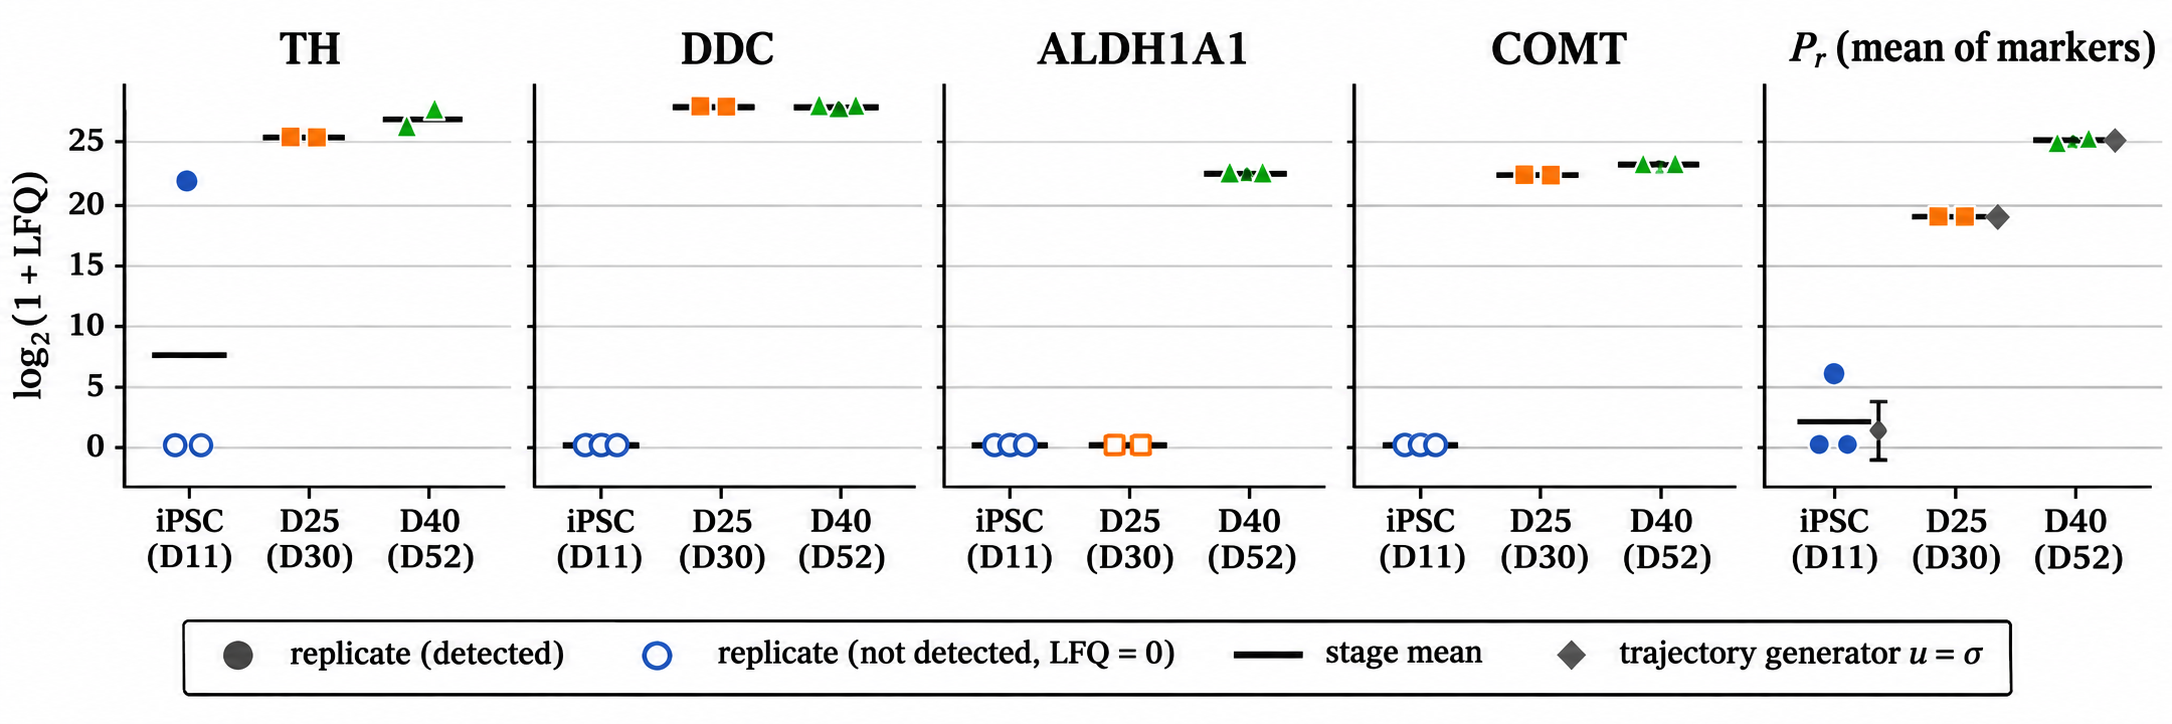
\includegraphics[width=0.90\linewidth]{images/fig_pr_replicates.png}
  \caption{\rtag{R2.11}\textcolor{red}{%
      \textbf{Individual proteomic CTRL replicates at each stage.}
      Columns show the four $\mathcal{G}_{Pr}$ markers and the
      replicate-level $Pr$ score on the $\log_{2}(1+\text{LFQ})$
      scale. Filled markers are quantified values; hollow markers
      are non-detections (LFQ $= 0$; in the $Pr$ panel, replicates
      with none of the four markers detected). Black bars are stage means.
      In the $Pr$ panel, grey diamonds with error bars show the
      mean $\pm$ s.d.\ of the distribution from which
      per-trajectory $Pr$ values are drawn
      (Section~\ref{sec:state}); at D11 this is the detection-floor
      anchor $\mathcal{N}(0, \sigma_{\text{D11}}/2)$ rather than the
      replicate mean. Stage is encoded by both x-position and
      marker shape. $n = 3/2/2$ replicates.}}
  \label{fig:replicates}
\end{figure*}

As a methodological robustness check, an interim
TH-abundance stratification was applied prior to receipt
of the canonical mapping.
All eight files exhibited TH log$_{2}$ LFQ intensities in
the range $[23.94,\,25.71]$, confirming \lang{that} all samples are
post-differentiation DA neurons ($\text{TH} \approx 0$
in undifferentiated iPSCs).
Splitting at the median TH abundance assigned the four
lower-TH files (Skupin11--14) to the D30 reference stage
and the four higher-TH files (Skupin15--18) to D52,
yielding $n = 4$ replicates per stage by pooling CTRL and
PINK1 (PINK1 affects TH by $\approx$10--20\%, smaller than
the $\approx 1$ log$_{2}$ inter-stage difference).

\begin{table*}[!htbp]
  \caption{%
    Proteomics marker set $\mathcal{G}_{Pr}$ curation
    (\lang{canonical sample mapping of the original authors}).
    Only markers with a confirmed monotonically increasing
    abundance across iPSC $\to$ D25 $\to$ D40 were retained.
    Per-stage values are log$_{2}$ LFQ intensities from
    the canonical CTRL-only proteinGroups;
    n/d = not detected by standard whole-cell-lysate LFQ.
    \rev{R2.4}{Values are means of $\log_{2}(1+\text{LFQ})$ over
      the stage's CTRL replicates; 0.00 means the protein is
      present in the table but has LFQ $= 0$ (not quantified) in
      every replicate of that stage, whereas n/d means it is absent
      from the table altogether. The iPSC value of TH (7.32) comes
      from a single replicate (21.97) averaged with two
      non-detections (Table~\ref{tab:replicates}).}}
  \label{tab:gpr}
  \centering
  \scalebox{0.79}{
    \begin{tabular}{lcccccl}
      \toprule
      Marker & iPSC & D25 & D40 & Verdict & Decision
      & Biological role \\
      \midrule
      TH
      & 7.32 & 25.43 & 26.79
      & $\uparrow$ monotonic
      & \textbf{Included}
      & Rate-limiting DA-synthesis enzyme \\
      DDC
      & 0.00 & 28.05 & 27.90
      & $\uparrow$ across stages\textsuperscript{$*$}
      & \textbf{Included}
      & DOPA decarboxylase (AADC) \\
      ALDH1A1
      & 0.00 & 0.00  & 22.50
      & sharp late-stage rise
      & \textbf{Included}
      & A9-DA subtype marker; PD-vulnerable \\
      COMT
      & 0.00 & 22.42 & 23.14
      & $\uparrow$ monotonic
      & \textbf{Included}
      & DA catabolism; rises with neuronal activity \\
      \midrule
      FOXA2
      & 0.00 & 11.09 & 0.00
      & non-monotonic
      & Excluded
      & Floor-plate TF; silenced by D40 \\
      NR4A2
      & n/d  & n/d   & n/d
      & ---
      & Excluded
      & Nuclear TF; below LFQ detection limit\textsuperscript{$\dagger$} \\
      PITX3
      & n/d  & n/d   & n/d
      & ---
      & Excluded
      & Nuclear TF; below LFQ detection limit\textsuperscript{$\dagger$} \\
      LMX1B
      & n/d  & n/d   & n/d
      & ---
      & Excluded
      & Nuclear TF; below LFQ detection limit\textsuperscript{$\dagger$} \\
      KCNJ6
      & n/d  & n/d   & n/d
      & ---
      & Excluded
      & Membrane channel; requires enrichment protocol \\
      \bottomrule
      \multicolumn{7}{l}{%
        \textsuperscript{$*$}DDC D25$\to$D40 plateau
        $\leq 0.15$ log$_{2}$ units --- within replicate noise;
        three-stage trajectory treated as monotonic.} \\
      \multicolumn{7}{l}{%
        \textsuperscript{$\dagger$}Absence confirmed in
        Cavarischia-Rega et al.~\cite{cavarischia2024proteome}
        (9,409 protein groups, \texttt{PXD050991}) ---
        \lang{a limitation of the MS method}.}
    \end{tabular}}
\end{table*}

% -----------------------------------------------------------------
\subsection{\textbf{Multi-omics state construction}}
\label{sec:state}

As shown in Figure~\ref{fig:pipeline} (Layer~2),
transcriptomic and proteomic inputs are harmonised into
a unified three-dimensional bounded state vector:
%
\begin{equation}
  \mathbf{s}_{t} = [P_{t},\; D_{t},\; Pr_{t}] \in [0,1]^{3}
  \label{eq:state}
\end{equation}

Pluripotency score $P_{t}$:
%
\begin{equation}
  P_{t}^{\text{raw}} =
    \frac{1}{|\mathcal{G}_{P}|}
    \sum_{g \in \mathcal{G}_{P}} \log\!\bigl(1 + \text{expr}_{t}(g)\bigr)
  \label{eq:P}
\end{equation}

Dopaminergic score $D_{t}$:
%
\begin{equation}
  D_{t}^{\text{raw}} =
    \frac{1}{|\mathcal{G}_{D}|}
    \sum_{g \in \mathcal{G}_{D}} \log\!\bigl(1 + \text{expr}_{t}(g)\bigr)
  \label{eq:D}
\end{equation}

\textbf{Proteomics score $Pr_{t}$:}
A curated marker set $\mathcal{G}_{Pr}$ was constructed by
retaining only proteins with a confirmed monotonically
increasing abundance across iPSC $\to$ D25 $\to$ D40 in
the \lang{canonical \texttt{proteinGroups} table}~\cite{novak2022single}, consistent with
dopaminergic maturation (Table~\ref{tab:gpr}).
This yielded:
%
\begin{equation}
  \mathcal{G}_{Pr} =
    \{\text{TH},\;\text{DDC},\;\text{ALDH1A1},\;\text{COMT}\}
  \label{eq:gpr}
\end{equation}
%
\begin{revblock}{R2.2,R2.14}
  \textbf{Rationale and adequacy of $\mathcal{G}_{Pr}$:}
  The candidate list was fixed \textit{a priori} from DA-neuron
  biology (Table~\ref{tab:gpr}), and markers were then retained
  only if they were quantified and rose with differentiation.
  The four retained proteins span the dopamine metabolic
  pathway of a functional DA neuron:
  TH converts tyrosine to L-DOPA and is the rate-limiting step of
  dopamine synthesis;
  DDC (aromatic L-amino acid decarboxylase) converts L-DOPA to
  dopamine;
  ALDH1A1 marks the A9 substantia nigra subtype that degenerates
  first in Parkinson's disease;
  and COMT degrades synaptic dopamine.
  $Pr$ therefore measures whether the cells have acquired the
  \textit{enzymatic machinery} of dopamine synthesis and turnover
  --- a functional property that the transcriptomic $D$ score,
  which mixes enzymes with transcription factors (LMX1A, FOXA2)
  and receptor/transporter genes, does not isolate at the protein
  level.
  The set does not represent all of DA identity: the defining
  transcription factors (NR4A2, PITX3, LMX1B) and the membrane
  channel KCNJ6 are below the detection limit of whole-cell
  label-free proteomics (Table~\ref{tab:gpr}), and the dopamine
  transporter (SLC6A3) is not quantified. $Pr$ is thus a marker
  of DA-pathway maturation rather than a complete DA-identity
  score; this is listed as a limitation in
  Section~\ref{sec:limitations}.
\end{revblock}
%
\begin{equation}
  Pr_{t}^{\text{raw}} =
    \frac{1}{|\mathcal{G}_{Pr}|}
    \sum_{p \in \mathcal{G}_{Pr}} \log_{2}\!\bigl(1 + a_{t}(p)\bigr)
  \label{eq:Pr}
\end{equation}
%
where $a_{t}(p)$ is the MaxQuant LFQ intensity of protein $p$
at stage $t$.
Per-stage means were computed over the canonical CTRL
replicates (D11: $\mu = 1.83 \pm 3.17$, $n = 3$;
D30: $\mu = 18.97 \pm 0.01$, $n = 2$;
D52: $\mu = 25.08 \pm 0.25$, $n = 2$; log$_{2}$ LFQ scale).

\begin{revblock}{R1.2,R2.6,AC}
  \textbf{Assigning $Pr$ to trajectories:}
  Proteomics and scRNA-seq were measured on different cells, so
  no cell has a measured $Pr$ value. Each trajectory $i$ instead
  receives, at each stage $t$, one value drawn independently of
  its $P$ and $D$ values:
  \begin{equation}
  Pr^{(i)}_{t} \sim
  \begin{cases}
    \mathcal{N}\bigl(\mu_{t},\, \sigma_{t}\bigr),
      & t \in \{\text{D30}, \text{D52}\},\\[2pt]
    \mathcal{N}\bigl(0,\, \sigma_{\text{D11}}/2\bigr),
      & t = \text{D11},
  \end{cases}
  \label{eq:prsample}
  \end{equation}
  with $(\mu_{t}, \sigma_{t})$ the replicate statistics above.
  D11 is anchored at the detection floor rather than at its
  replicate mean because two of the three iPSC replicates contain
  no $\mathcal{G}_{Pr}$ marker at all and the mean of 1.83 is
  produced by a single TH detection in one replicate
  (Table~\ref{tab:replicates}); a pre-DA stage is expected to sit
  at the floor of the DA-pathway axis. The floor keeps a small
  spread, half the D11 replicate standard deviation
  ($\sigma = 1.59$), so that D11 values are not all identical.
  This anchor was used for every result reported, and it
  replaces the description $\mathcal{N}(\mu_{\text{stage}},
\sigma_{\text{stage}})$ for all stages given in the original
  submission;
  it is shown alongside the replicate data in
  Figure~\ref{fig:replicates}, and because D11 ($\approx 0$)
  and D30 ($\approx 19$) are far apart on the $Pr$ axis under
  either choice, it does not affect the stage ordering that the
  analyses rely on.
  The random draws are made with the run's seed
  (Section~\ref{sec:multiseed}).
  Within-stage sampling preserves a plausible within-stage
  spread; the deterministic ablation
  (Section~\ref{sec:ablations}), which sets every value to the
  stage centre, shows that this spread carries no additional
  signal.
\end{revblock}

\textbf{Normalisation:}
\rev{R2.6,AC}{The $Pr$ score is scaled to $[0,1]$ using min-max
  bounds computed from the training-split trajectories only,
  refitted for every seed:}
%
\begin{equation}
  z^{\text{norm}} =
    \operatorname{clip}\!\left(
      \frac{z - z^{\text{tr}}_{\min}}
           {z^{\text{tr}}_{\max} - z^{\text{tr}}_{\min}},\;
      0,\; 1
    \right)
  \label{eq:norm}
\end{equation}
\begin{revblock}{R2.6,AC}
  $P$ and $D$ enter already scaled by the fixed cell-population
  bounds of the baseline (Section~\ref{sec:baseline}); these
  bounds are not refitted per split.
  \textbf{Leakage control.} Three facts limit what the test
  trajectories can contribute to training.
  \textit{(i)} The split is made over whole trajectories, so no
  test trajectory, and none of its three states, is seen during
  training.
  \textit{(ii)} The only fitted preprocessing on $Pr$ (its
  min-max bounds) uses training trajectories only.
  \textit{(iii)} The $P$/$D$ bounds are two fixed constants per
  axis computed without stage labels over all 161,584 cells; a
  fixed monotone rescaling applied identically to every split
  cannot carry label information from test to training data.
  What is shared between training and test trajectories by
  design is the stage-level proteomic distribution of
  Eq.~\eqref{eq:prsample}: every trajectory's $Pr$ at a given
  stage is drawn from the same $(\mu_{t}, \sigma_{t})$, which is
  estimated from the proteomic replicates and from no
  trajectory. Because these stage statistics define where each
  stage sits on the $Pr$ axis, Task~A measures how separable the
  stages are under this representation, not out-of-sample
  prediction of unseen biology (Sections~\ref{sec:loro}
  and~\ref{sec:pronly}).
\end{revblock}

\textbf{Trajectory assembly:}
$N = 200$ trajectories were assembled by sampling one cell
per timepoint:
%
\begin{equation}
  \mathbf{x}^{(i)} =
    \bigl(\mathbf{s}^{(i)}_{11},\;
           \mathbf{s}^{(i)}_{30},\;
           \mathbf{s}^{(i)}_{52}\bigr),
  \quad i = 1,\ldots,200
  \label{eq:traj}
\end{equation}
%
yielding a tensor of size $200 \times 3 \times 3$.
\begin{revblock}{R1.2}
  Concretely, for each trajectory $i$ one cell was drawn
  uniformly at random from the untreated D11 cells, one from
  the D30 cells and one from the D52 cells, independently of
  each other and of the other trajectories; the cell's $P$ and
  $D$ scores form $\mathbf{s}^{(i)}_{t}$ and $Pr^{(i)}_{t}$ is
  added by Eq.~\eqref{eq:prsample}.
  scRNA-seq destroys the cell, so the three cells of a trajectory
  are different cells and a trajectory is a population-level
  pseudo-trajectory, not a lineage-traced path of one cell.
  The 200 $(P, D)$ trajectories are the published tensor of the
  baseline study~\cite{kanu2026transformer} and are identical in
  every run; they are not re-sampled per seed.
\end{revblock}
Trajectories were split into train/validation/test sets
of 140/30/30\rev{R1.4,R2.9}{; the split is redrawn for each of
  the 20 seeds (Section~\ref{sec:multiseed}), and the reference
  seed 42 is the seed used by} the 2D baseline described in
Section~\ref{sec:baseline}.

% -----------------------------------------------------------------
\subsection{\textbf{DLT-based provenance for reproducibility}}
\label{sec:dlt}

Multi-source computational pipelines face a documented
reproducibility challenge: dataset versions change silently
and preprocessing decisions are frequently underreported,
preventing independent verification of published
results~\cite{kanu2024blockchain}.
As illustrated by the provenance bar in
Figure~\ref{fig:pipeline}, we address this by recording
immutable data fingerprints at every ingestion and
processing step on a distributed ledger.

A \texttt{MultiOmicsProvenance} smart contract was deployed
on the PureChain mainnet (chain ID \texttt{900520900520},
gas-free EVM, RPC \texttt{https://purechainnode.com}) at
address \texttt{0xFA954E93c389D54B05FBA832276B7C7a42bAeD51}\rev{R2.24}{
  (compiler and deployment settings: Supplementary Table~S1)}.
Each data ingestion event (Layer~1, Figure~\ref{fig:pipeline})
registers: source name and URL, dataset version, access date,
SHA-256 hash of the raw downloaded file, the list of markers
used, the normalisation procedure applied, and the Git commit
hash of the processing pipeline.
A linked processed record (Layer~2, Figure~\ref{fig:pipeline})
commits the SHA-256 of the output score matrix to the same
pipeline version.
The \texttt{verifyIngestion} contract function enables any
researcher to independently verify data integrity by
comparing their local file hash against the immutable
on-chain record.
Integrity guarantees hold under the proof-of-authority-and-association (PoA$^2$)~\cite{kanu2026offline} trust
model of the permissioned chain; the recorded confirmation
depth quantifies transaction finality rather than a
proof-of-work attack cost.

\begin{revblock}{R1.11,R2.16}
  For a biomedical reader the ledger can be thought of as a
  public, tamper-evident lab notebook for data files. A SHA-256
  fingerprint is a short code computed from every byte of a
  file; changing a single byte produces a completely different
  code. When the pipeline downloads the scRNA-seq or proteomics
  data, it writes the fingerprint, the dataset version, and the
  exact code version (Git commit) to the ledger, where entries
  cannot be edited or deleted afterwards. A reader who wants to
  reproduce or audit the results recomputes the fingerprint of
  their own copy and calls \texttt{verifyIngestion}: a match
  proves they are using byte-identical inputs and code; a
  mismatch reveals at once that a dataset was silently updated,
  re-processed differently, or substituted. This matters most in
  multi-source pipelines such as this one, where two datasets
  from different laboratories, a locally re-processed
  proteomics table, and several derived score files must all
  stay consistent. The layer certifies \textit{which} data and
  code produced a result; it does not certify that the analysis
  itself is correct.
\end{revblock}

% -----------------------------------------------------------------
\subsection{\textbf{Evaluation protocol}}
\label{sec:eval}

The evaluation suite (Figure~\ref{fig:pipeline}, Layers~3--4)
benchmarks three model families on two tasks under identical
splits and normalisation, with permutation nulls, a
leave-one-replicate-out probe, and a single-feature baseline
to distinguish real proteomic signal from \lang{artefacts of
  model capacity or of state construction}.

\subsubsection{Tasks}

\textbf{Task A --- Stage separability:}
Given a state vector $\mathbf{s}_{t} \in [0,1]^{k}$
($k = 2$ for 2D, $k = 3$ for 3D), predict the differentiation
stage label $y \in \{\text{D11, D30, D52}\}$.
Performance is reported as macro-averaged F1.
This task is framed as a separability check on the state
space --- a test of whether the proteomic axis carries
stage-discriminating information that the transcriptomic
axes do not --- rather than as a predictive contribution in
itself; the diagnostics of
Sections~\ref{sec:loro}--\ref{sec:pronly} establish what the
resulting separability does and does not demonstrate.

\textbf{Task B --- Trajectory prediction:}
Given the two-step input context
$[\mathbf{s}_{11}, \mathbf{s}_{30}] \in [0,1]^{2 \times k}$,
predict the late-stage state $\mathbf{s}_{52}$.
Performance is reported as mean absolute error (MAE),
averaged across state dimensions:
%
\begin{equation}
  \text{MAE} =
    \frac{1}{n\textcolor{red}{k}}
    \sum_{i=1}^{n}
    \bigl\lVert \mathbf{s}^{(i)}_{52} -
                \hat{\mathbf{s}}^{(i)}_{52} \bigr\rVert_{1}
  \label{eq:mae}
\end{equation}
\rev{AC}{where $k$ is the number of state dimensions, so that
  the 2D and 3D errors are both per-dimension averages and
  directly comparable.}
%
A per-dimension decomposition is also reported
(Section~\ref{sec:results}) so that the contribution of the
added $Pr$ dimension to the aggregate MAE is separated from
any change in the $P$ and $D$ forecasts.

\subsubsection{Models}

Three model families were evaluated under identical splits
and normalisation for both the 2D baseline and 3D extension
(Figure~\ref{fig:pipeline}, Layer~3):
\textit{(i)} \rev{AC}{a linear model: multinomial logistic
  regression for Task~A and} Ridge regression ($\alpha = 1.0$)
\rev{AC}{for Task~B},
\textit{(ii)} Random Forest (\rev{AC}{200 estimators for both
  tasks}), and
\textit{(iii)} a Transformer digital twin with the
architecture described in Section~\ref{sec:baseline}:
4 encoder layers, 4 attention heads,
$d_{\text{model}} = 128$, feedforward dimension 512,
dropout 0.1, trained with Adam ($\text{lr} = 10^{-3}$)
and early stopping on validation loss (patience 10).
The only change between 2D and 3D conditions is the
per-token input feature width.

\subsubsection{Multi-seed protocol and significance testing}
\label{sec:multiseed}

To replace single-seed point estimates with interval
estimates, the full Task~A and Task~B benchmark is run across
20 seeds \rev{R1.4,R2.9}{(42--61)}. Each seed independently parameterises the
per-trajectory $Pr$ sampling of \rev{AC}{Eq.~\eqref{eq:prsample}}, the
train/validation/test split, the permutation-null shuffles,
and every model's initialisation. All tabulated quantities
are reported as mean $\pm$ standard deviation across seeds.
\rev{R1.4,R2.9}{The seed does \textit{not} change the 200
  $(P, D)$ trajectories, which are fixed (Section~\ref{sec:state}),
  or the proteomic stage statistics.}
For the 2D$\to$3D Task~B MAE reduction, a one-sided paired
Wilcoxon signed-rank test (\rev{AC}{$\text{MAE}_{3\text{D}} <
\text{MAE}_{2\text{D}}$}) is applied to the 20 per-seed paired
differences within each model family\lang{;} Cohen's $d_{z}$ is
reported as the paired effect size, and Holm--Bonferroni
correction is applied across the three model families.

\begin{revblock}{R2.9,R1.4}
  \textbf{Independence of seeds and choice of test.}
  Within a seed, the 2D and 3D models share the same split and
  the same trajectories, so the two MAEs form a natural pair and
  the per-seed difference removes split-to-split variation; this
  is why a paired test is used. Across seeds the draws are made
  with independent random streams, but the runs are not fully
  independent observations: they reuse the same 200 $(P, D)$
  trajectories, the same proteomic statistics, and overlapping
  training sets. The Wilcoxon signed-rank test was chosen
  because it does not assume the 20 paired differences are
  normally distributed, which cannot be checked reliably at
  $n = 20$. Its $p$-values should therefore be read as evidence
  that the 2D$\to$3D difference is robust to the random choices
  of the pipeline (split, $Pr$ draw, initialisation), not as
  inference about new biological samples or new datasets.
  To report the size of the effect with its uncertainty, a 95\%
  confidence interval for the mean paired MAE difference and for
  the relative change is also computed by percentile bootstrap
  over seeds (10,000 resamples, seeds resampled in pairs).
\end{revblock}

\subsubsection{Permutation nulls}

Two permutation nulls were computed to distinguish real
proteomic signal from added model capacity
(red dashed arrow, Figure~\ref{fig:pipeline}):
%
\begin{itemize}
  \item \textbf{perm\_across}: $Pr$ values are shuffled
  globally across all 600 cell-stage observations,
  destroying the stage--$Pr$ coupling while preserving
  the overall $Pr$ distribution.
  This is the appropriate null for Task~A: it tests whether
  the separability lift reflects genuine stage--$Pr$
  coupling rather than added model capacity.
  \item \textbf{perm\_within}: $Pr$ values are shuffled
  independently within each stage, destroying cell-level
  $Pr$ associations while preserving per-stage marginals.
  This is the appropriate null for Task~B: it tests whether
  cell-level $Pr$ variation contributes beyond the
  per-stage marginal structure.
\end{itemize}

\subsubsection{Leave-one-replicate-out probe}
\label{sec:loro}

Because $Pr_{t}$ is constructed from per-stage means computed
over the canonical CTRL replicates ($n = 3/2/2$), and those
same stage means inform the stage label, the permutation
nulls alone cannot establish that Task~A separability
generalises to a replicate that did not contribute to the
stage mean against which it is classified. A
leave-one-replicate-out (LORO) probe tests this directly.
For each of the seven canonical CTRL replicates $s$ held out
in turn: the affected stage mean and standard deviation
$(\mu_{\text{stage}}, \sigma_{\text{stage}})$ are recomputed
from the remaining replicates only; the trajectory tensor is
regenerated; training-split-only min-max bounds
(Eq.~\eqref{eq:norm}) are refit on $Pr$; and Task~A is
re-evaluated. Macro F1 is reported as mean $\pm$ standard
deviation across the seven folds.
Because two stages contribute only two replicates each, every
held-out fold leaves a single replicate defining the stage
mean; the probe is therefore a consistency check under the
available replicate structure rather than a powered
cross-validation, and is reported as such.
\rev{R1.3}{In particular, LORO is not an external validation:
  all seven replicates come from one laboratory, one cell line
  and one differentiation protocol, and a held-out replicate is
  still classified against trajectories generated from the same
  study. It shows that the result does not hinge on any single
  replicate; it cannot show that the result transfers to
  independent datasets.}

\subsubsection{Single-feature ($Pr$-only) baseline}
\label{sec:pronly}

To locate where the Task~A signal resides, a classifier is
trained on the $Pr$ axis alone (a single feature) under the
same splits and normalisation, and reported alongside the 2D
and 3D conditions. If the $Pr$-only baseline matches the 3D
separability, then for stage separability the
multidimensional state offers nothing beyond the single
monotonic proteomic axis; the multi-omics value of the 3D
state then rests on \rev{AC}{Task~B and on the stage information
  that $Pr$ adds}, not on Task~A capacity. This decomposition is
reported explicitly rather than left implicit.

\begin{figure*}[t]
  \centering
  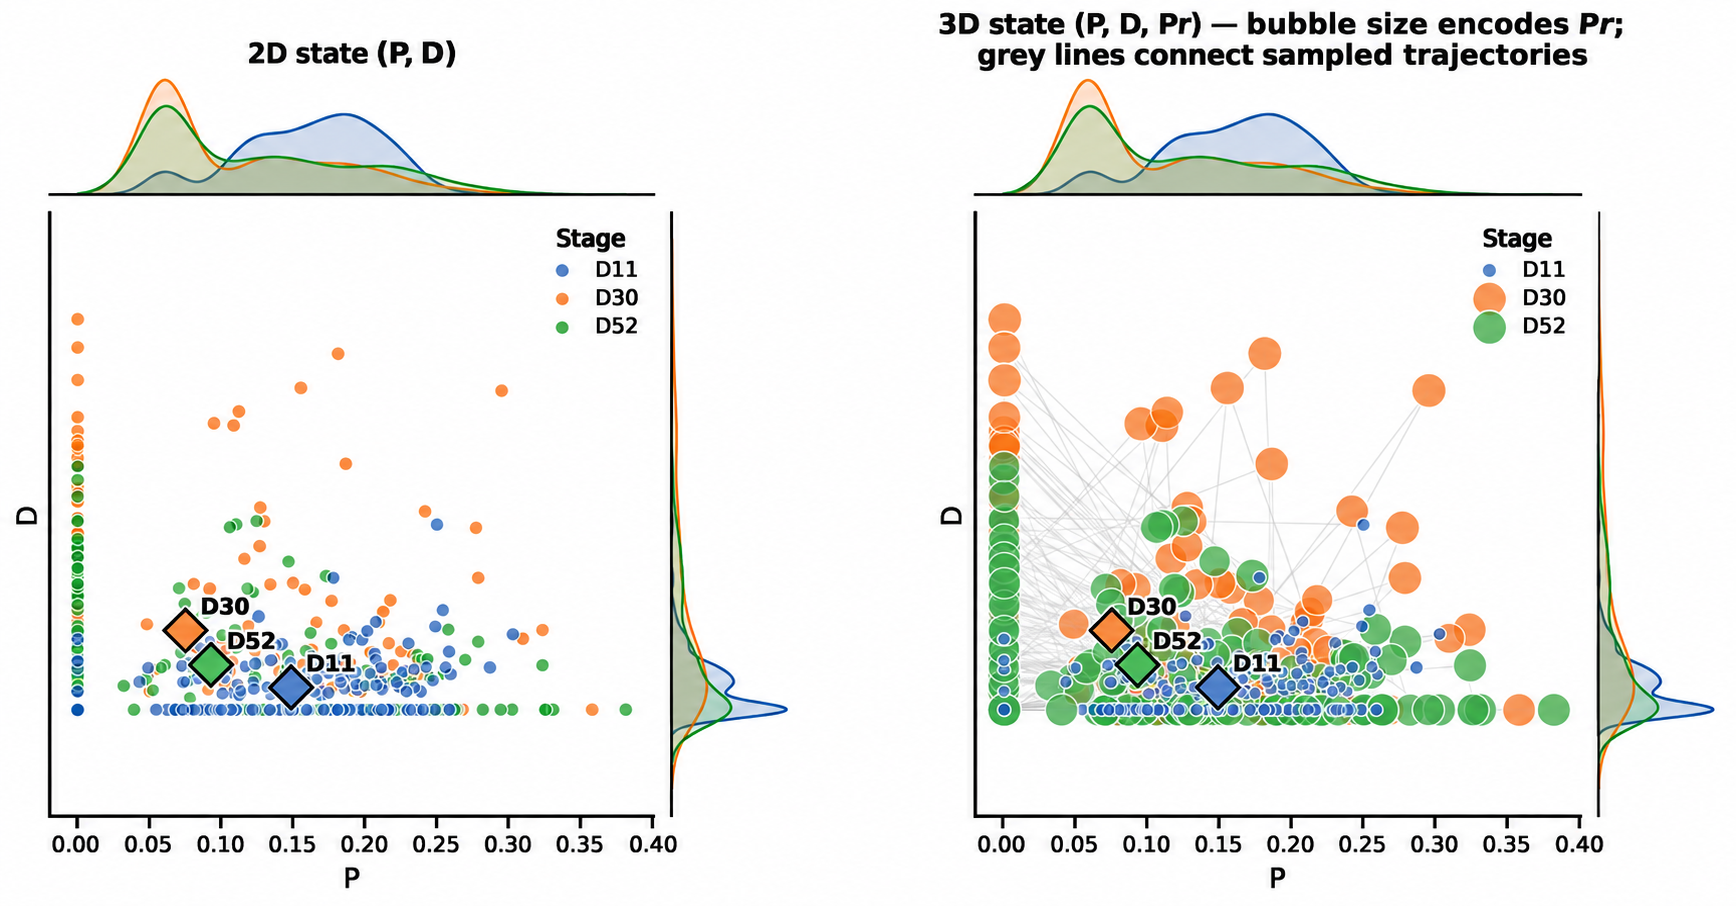
\includegraphics[width=0.75\linewidth]{images/fig2_2d_vs_3d.png}
  \caption{%
    \textbf{2D versus 3D state space representation across
      differentiation stages D11, D30, and D52.}
    \textit{Left:} transcriptomic-only 2D state $(P, D)$
    showing substantial overlap between D11 and D30 in both
    the scatter and marginal density plots.
    \textit{Right:} proteomics-integrated 3D state $(P, D, Pr)$
    where bubble size encodes $Pr$; grey lines connect sampled
    trajectories across timepoints.
    Stage centroids are shown as labelled diamonds.
    Addition of the proteomic axis resolves the stage ambiguity
    present in the 2D projection.
    $n = 200$ sampled trajectories; colours indicate stage
    identity (D11 blue, D30 orange, D52 green).
    \rev{R1.7}{This figure shows the state representations
      only; model performance under the 2D, 3D, $Pr$-only and
      permutation-null conditions is reported in
      Figure~\ref{fig:benchmark} and Table~\ref{tab:taska}. The
      right panel uses the D11 detection-floor anchor of
      Eq.~\eqref{eq:prsample}.}}
  \label{fig:scatter}
\end{figure*}

\subsubsection{Sensitivity ablations}
\label{sec:ablations}

Two ablations interrogate key design choices
(Figure~\ref{fig:pipeline}, Layer~4 ablations box).
\textit{(i)} \textbf{Deterministic $Pr$}: each trajectory
cell receives the exact stage mean ($\sigma = 0$), testing
whether the stochastic sampling in \rev{AC}{Eq.~\eqref{eq:prsample}}
introduces or removes signal beyond the per-stage marginal.
\textit{(ii)} \textbf{4D $+ K_{t}$}: a transcript-derived
kinase-pathway activity score is added as a fourth state
dimension, computed as the mean log-normalised expression
of 13 canonical MAPK and PI3K/AKT target genes
(\textit{FOS, JUN, EGR1, DUSP1, DUSP6, MYC, CCND1,
  FOXO3, BCL2, MDM2, CDKN1A, GSK3B, TSC2})
on the Jerber transcriptome~\cite{jerber2021population}.
This tests whether a transcript-derived phospho-pathway
proxy adds value beyond the measured 3D state.

%% ============================================================
%%  REQUIRED PREAMBLE (add to main.tex if not already present)
%%  \usepackage{booktabs}
%%  \usepackage{siunitx}
%%  \usepackage{graphicx}
%%  \usepackage{subcaption}
%%  \graphicspath{{figures/}}   % folder where your .png/.pdf files live
%% ============================================================

%% ============================================================
%%  RESULTS
%% ============================================================
\section{Results}
\label{sec:results}

% -----------------------------------------------------------------
\subsection{\textbf{State space characterisation}}
\label{sec:res_state}

Figure~\ref{fig:scatter} contrasts the 2D transcriptomic state
$(P, D)$ and the 3D proteomics-integrated state $(P, D, Pr)$
across differentiation stages D11, D30, and D52.
In the 2D projection, D11 and D30 cells occupy overlapping
regions of the $(P, D)$ plane: pluripotency scores decline
from D11 to D52 ($\mu_{P}$: $0.72 \to 0.18 \to 0.06$),
while dopaminergic scores follow a non-monotonic trajectory
($\mu_{D}$: $0.12 \to 0.65 \to 0.44$), with a transient
peak at D30 that partially obscures the D30--D52 boundary.
Adding $Pr$ resolves this ambiguity: the proteomics score
increases monotonically across stages
(D11: $\mu_{Pr} = 1.83 \pm 3.17$;
D30: $18.97 \pm 0.01$;
D52: $25.08 \pm 0.25$; log$_{2}$ LFQ scale\rev{AC}{; replicate
  statistics, with D11 trajectories drawn at the detection floor
  of Eq.~\eqref{eq:prsample}}),
producing three visually non-overlapping clusters in 3D.
Marginal density plots confirm that stage separation along the
$P$-axis is similar between 2D and 3D; the critical gain is
along the $Pr$ axis, where all three stages are cleanly
separated from one another.
\rev{R1.13}{\textit{Takeaway (Fig.~\ref{fig:scatter}):} the
  transcriptomic plane confuses D11 with D30 and D30 with D52;
  the proteomic axis places the three stages at clearly different
  levels.}

% -----------------------------------------------------------------
\subsection{\textbf{Cross-modal orthogonality and trajectory
    coherence}}
\label{sec:res_orthog}

\begin{figure*}[!htbp]
  \centering
  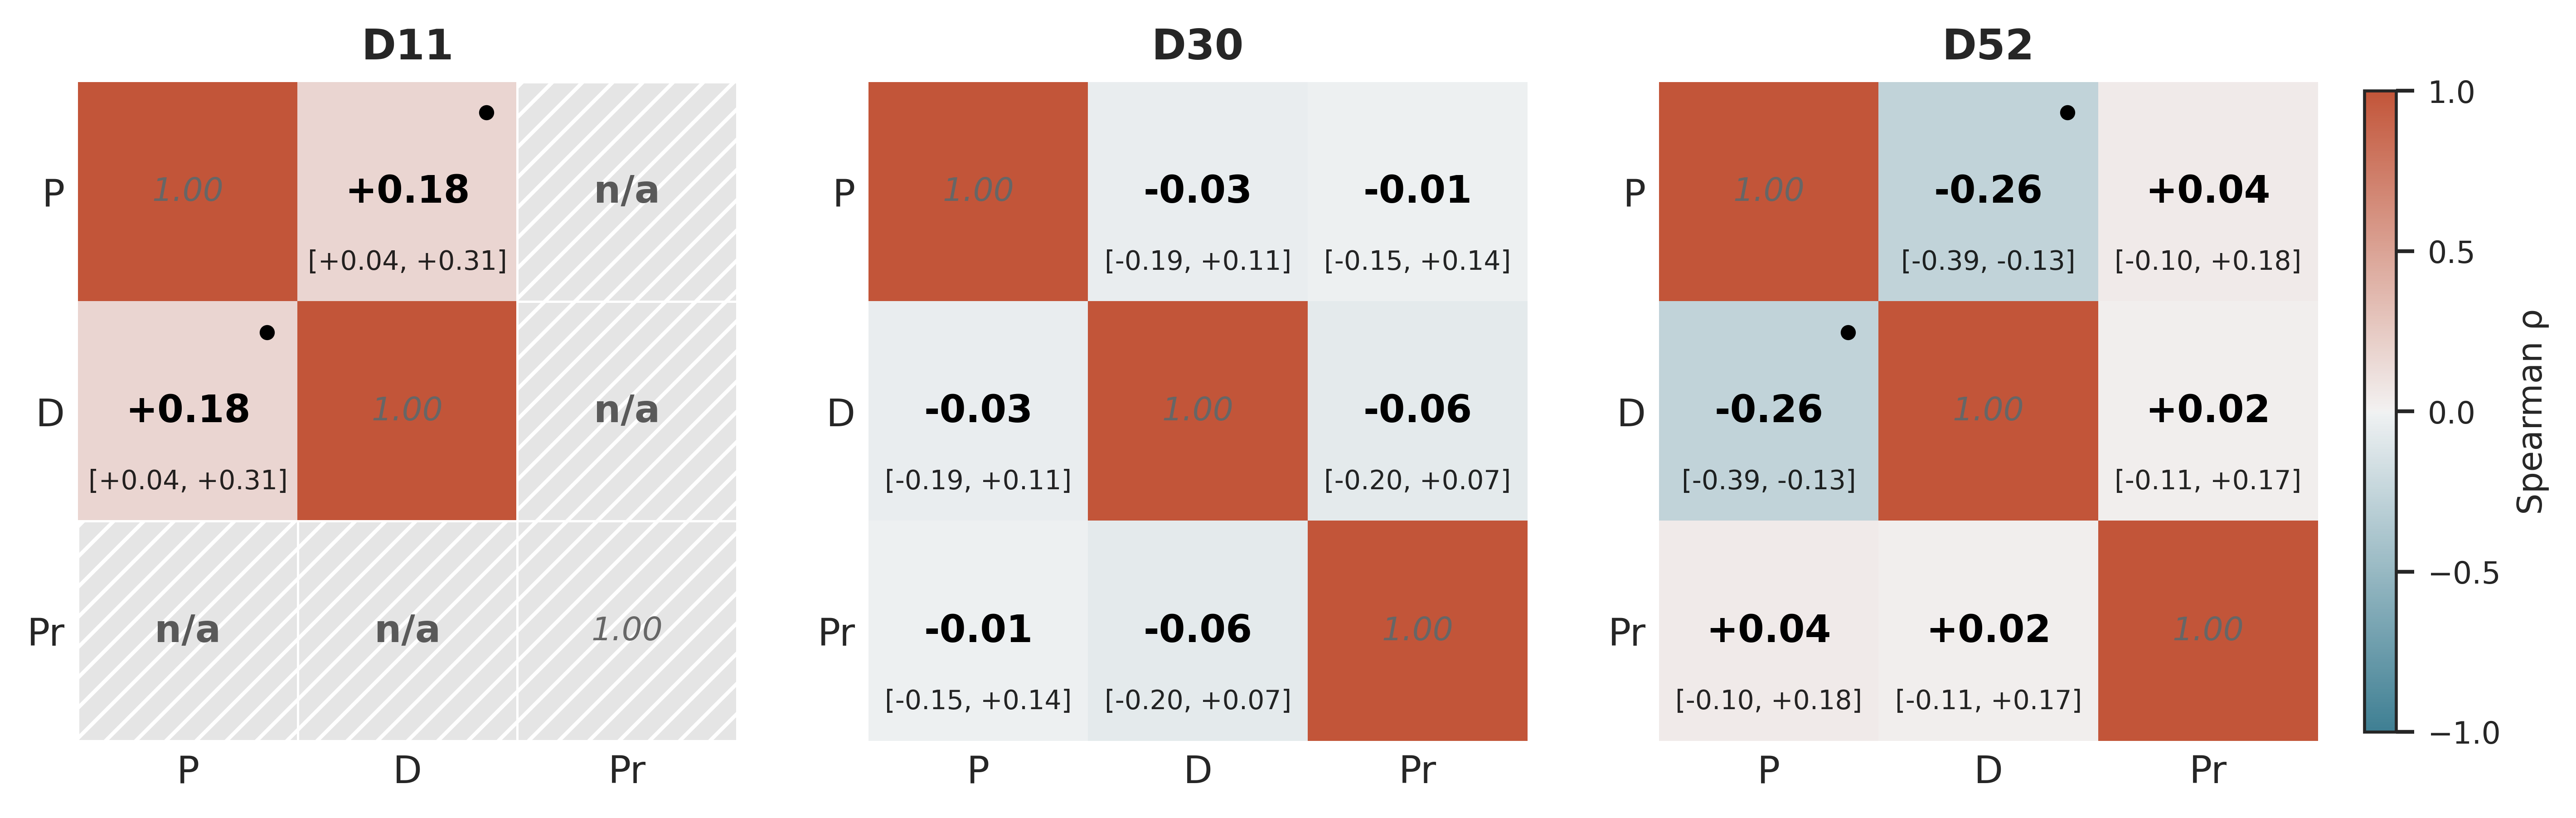
\includegraphics[width=0.70\linewidth]{images/fig3_correlations.png}
  \caption{%
    \textbf{Per-stage Spearman correlation matrices among
      $(P, D, Pr)$.}
    Each cell reports the Spearman $\rho$ estimate with 95\%
    bootstrap confidence interval ($n = 1{,}000$ resamples).
    All $Pr$ correlations at every stage have confidence
    intervals straddling zero ($|\rho| \leq 0.08$)\rev{AC}{, as
      expected because $Pr$ is drawn independently of $P$ and $D$
      within each stage (Eq.~\eqref{eq:prsample})}.}
  \label{fig:corr}
\end{figure*}

\begin{table}[!htbp]
  \caption{%
    Cross-modal Spearman correlations among $(P, D, Pr)$ per stage
    with bootstrap 95\% CIs ($n = 1{,}000$ resamples).
    All $Pr$ correlations have CIs straddling zero.}
  \label{tab:correlations}
  \centering
  \scalebox{0.70}{
    \begin{tabular}{lccc}
      \toprule
      Stage & $\rho(P,D)$ & $\rho(P,Pr)$ & $\rho(D,Pr)$ \\
      \midrule
      D11 & $+0.18$ & $-0.06$ & $-0.08$ \\
      D30 & $-0.03$ & $+0.03$ & $-0.00$ \\
      D52 & $-0.26$ & $-0.01$ & $-0.01$ \\
      \bottomrule
    \end{tabular}}
\end{table}

\begin{table}[!htbp]
  \caption{%
    Trajectory coherence
    $C^{(i)} = \cos(\mathbf{s}_{30} - \mathbf{s}_{11},\;
  \mathbf{s}_{52} - \mathbf{s}_{30})$, reported as a structural
    sanity check ($n = 200$ trajectories). The stochastic-$Pr$
    row is the meaningful one; the deterministic-$Pr$ row reaches
    the $+1$ ceiling by construction because $Pr$ is monotone
    across stages.}
  \label{tab:coherence}
  \centering
  \scalebox{0.70}{
    \begin{tabular}{lccc}
      \toprule
      State space & Mean & Std & Median \\
      \midrule
      2D $(P,D)$                  & $-0.502$ & $0.604$ & $-0.828$ \\
      3D $(P,D,Pr)$ stochastic    & $\mathbf{+0.998}$ & $0.002$ & $\mathbf{+0.999}$ \\
      3D $(P,D,Pr)$ deterministic & $+0.998$ & $0.002$ & $+0.999$ \\
      \bottomrule
    \end{tabular}}
\end{table}

Table~\ref{tab:correlations} and Figure~\ref{fig:corr} report
per-stage Spearman $\rho$ matrices among $(P, D, Pr)$ with
bootstrapped 95\% confidence intervals ($n = 1{,}000$ resamples).
At every stage, all pairwise correlations involving $Pr$ have
confidence intervals straddling zero ($|\rho| \leq 0.08$)\rev{AC}{;
  this is expected by construction (see below) and shows that the
  assembled state introduces no spurious within-stage coupling.
  The} between-stage $Pr$ gradient --- not
within-stage cross-modal coupling --- is what separates the
stages in Section~\ref{sec:res_bench}.
The mild P--D anticorrelation at D52 ($\rho = -0.26$,
95\% CI $[-0.39, -0.13]$) is consistent with the non-monotonic
D-axis behaviour of the 2D baseline described in
Section~\ref{sec:baseline}.

\begin{figure*}[!htbp]
  \centering
  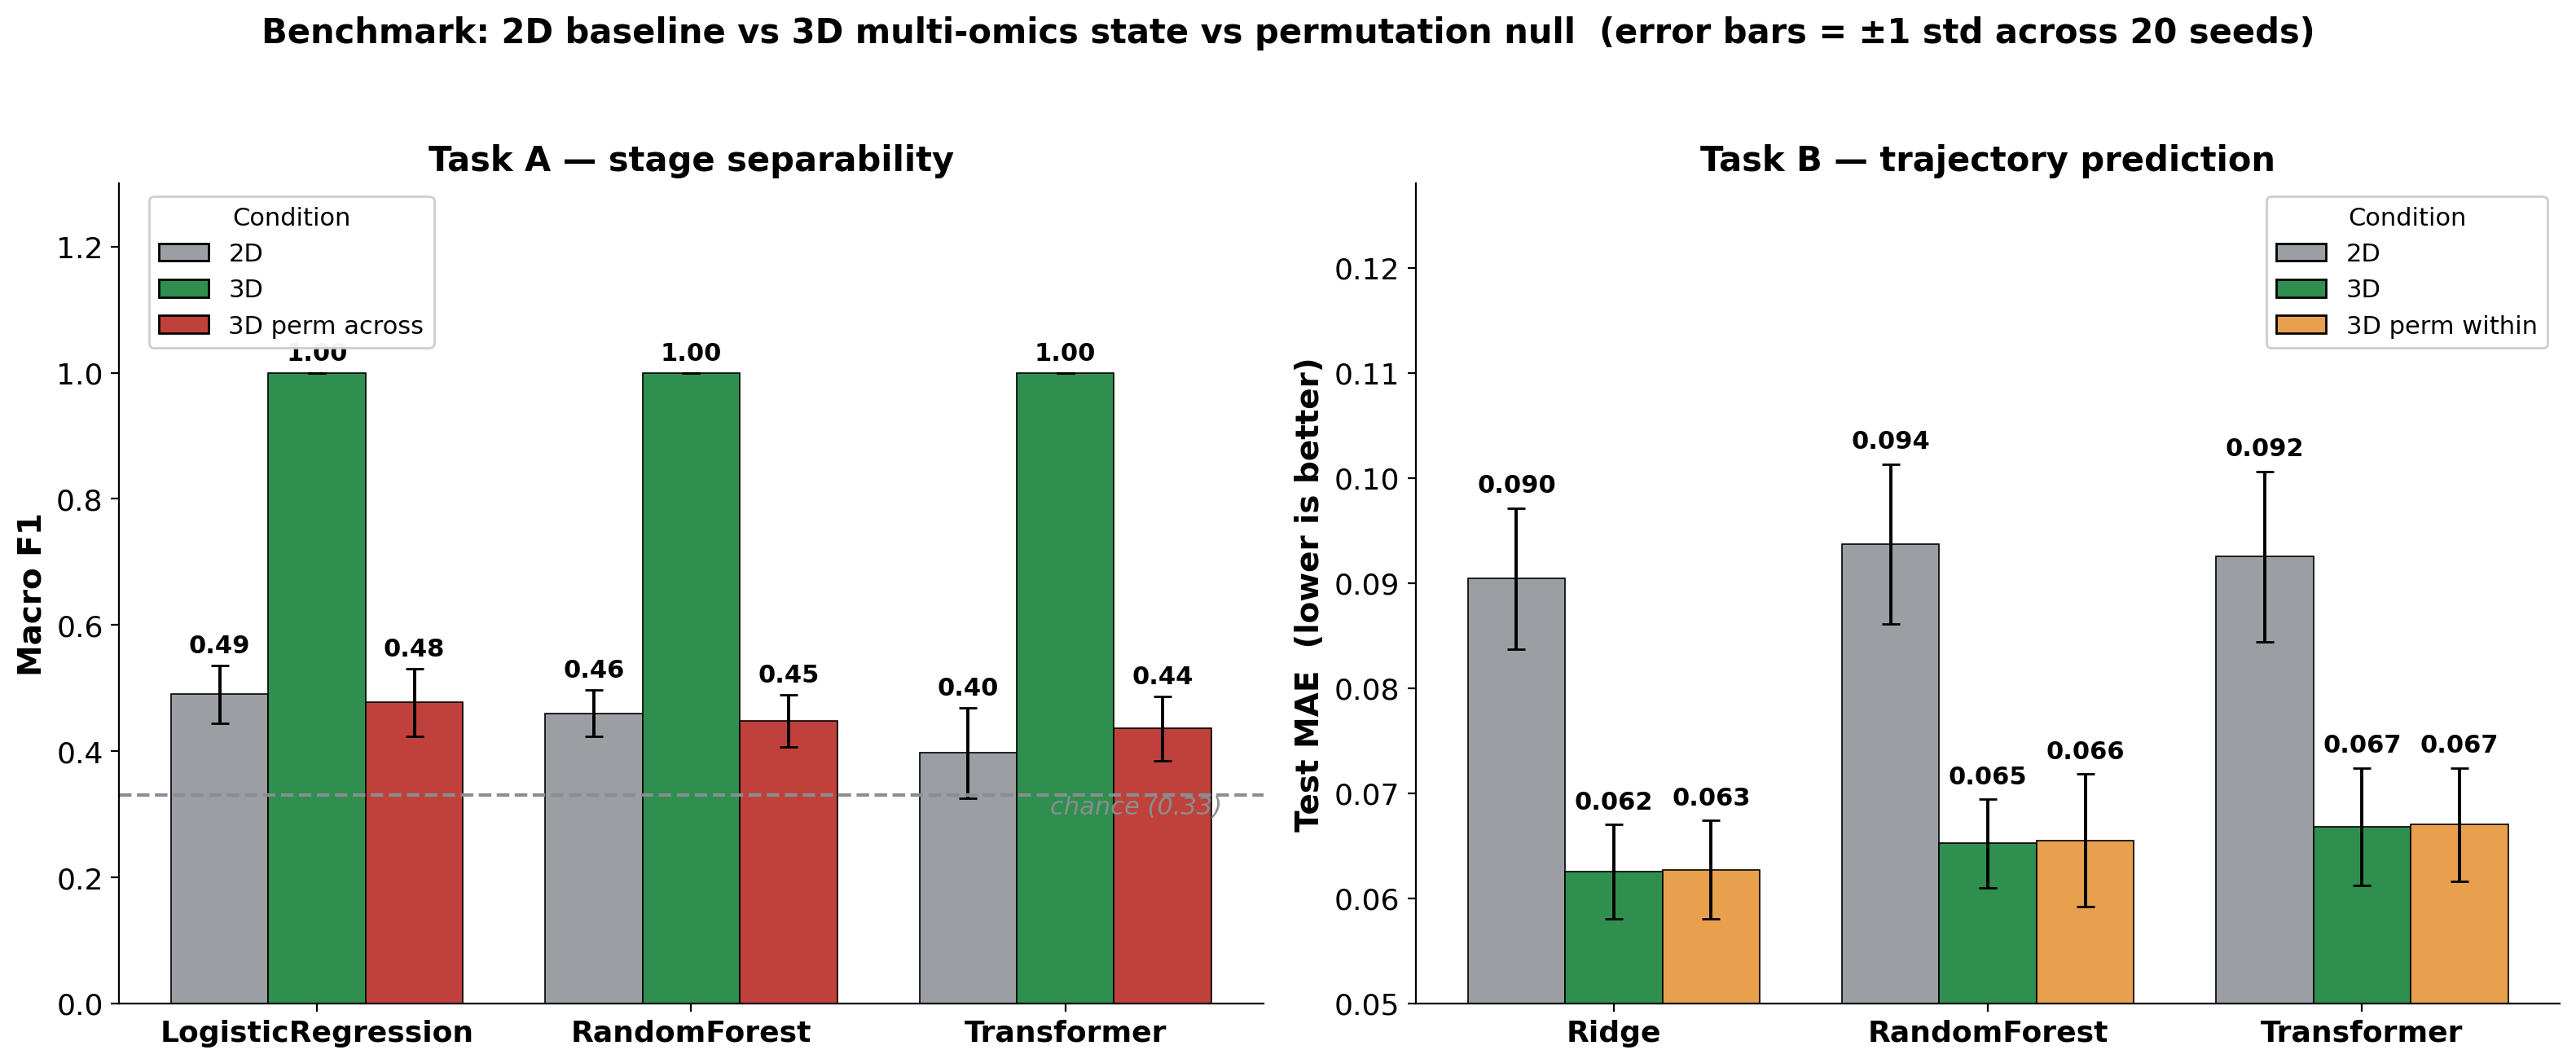
\includegraphics[width=0.85\linewidth]{images/fig4_benchmark.png}
  \caption{%
    \textbf{Benchmark performance under 2D and 3D state
      conditions with permutation nulls.}
    \textit{(A)} Task A macro F1 for stage separability.
    Dashed line marks three-class chance level (0.33).
    \textit{(B)} Task B MAE for trajectory prediction (lower
    is better); y-axis starts at 0.05 to highlight
    inter-condition differences.
    Bars show mean over 20 seeds; error bars show $\pm$ std.
    Grey = 2D baseline; green = 3D proteomics-integrated;
    red = \texttt{perm\_across} null (Task~A);
    amber = \texttt{perm\_within} null (Task~B).
    Collapse of 3D performance to near-chance under
    \texttt{perm\_across} confirms the separability lift
    arises from real proteomic-stage signal.
    $n = 30$ held-out test trajectories.
    \rev{R1.7}{Condition labels follow
      Section~\ref{sec:res_bench}: ``3D perm across'' is the
      Task~A null and ``3D perm within'' the Task~B null. The
      $Pr$-only and LORO conditions are not drawn because they
      equal the 3D bars exactly (F1 $= 1.000$ in every run); their
      values are in Table~\ref{tab:taska}. Panel~(B) shows the
      overall MAE; its per-dimension breakdown is in
      Table~\ref{tab:taskb_perdim}. Model labels: the linear model
      is logistic regression in (A) and Ridge regression in (B).}}
  \label{fig:benchmark}
\end{figure*}

Trajectory coherence, defined as the cosine similarity between
consecutive displacement vectors
$C^{(i)} = \cos(\mathbf{s}^{(i)}_{30} - \mathbf{s}^{(i)}_{11},\;
\mathbf{s}^{(i)}_{52} - \mathbf{s}^{(i)}_{30})$,
is reported in Table~\ref{tab:coherence} as a structural sanity
check rather than as evidence of model quality.
The 2D state yields strongly negative population-mean coherence
($\mu = -0.502$, median $= -0.828$), reflecting the
advance-then-retreat trajectory shape induced by the D-axis
peak at D30.
Adding $Pr$ drives mean coherence to $+0.998$ (median $+0.999$,
std $0.002$).
The near-ceiling value is structural: $Pr$ was curated to
include only markers with confirmed monotonically increasing
abundance across iPSC $\to$ D25 $\to$ D40, producing large
positive $Pr$ displacement vectors at both the D11$\to$D30 and
D30$\to$D52 transitions that dominate the cosine direction even
when the $D$ component dips.
Stochastic and deterministic $Pr$ sampling yield essentially
identical coherence, confirming \lang{that} the $+1$ ceiling reflects the
monotone stage structure of $Pr$ and not per-cell variance.
\rev{AC}{Coherence is therefore not used as evidence that $Pr$ is
  non-redundant.}
\rev{R1.13}{\textit{Takeaway (Fig.~\ref{fig:corr},
    Tables~\ref{tab:correlations}--\ref{tab:coherence}):} the
  assembled state introduces no within-stage coupling between
  $Pr$ and the transcriptomic axes, and the near-perfect
  coherence is a structural consequence of a monotone $Pr$; the
  evidence that $Pr$ complements $P$ and $D$ is the stage
  information it adds (Section~\ref{sec:res_taska}).}
\rev{AC}{Because $Pr$ is drawn independently of $P$ and $D$
  within each stage (Eq.~\eqref{eq:prsample}), the near-zero
  within-stage correlations are expected by construction; they
  confirm that the assembled state introduces no spurious
  coupling, while the biological complementarity of $Pr$ rests
  on the between-stage information it carries.}

% -----------------------------------------------------------------
\subsection{\textbf{Benchmark performance}}
\label{sec:res_bench}

Figure~\ref{fig:benchmark} and
Tables~\ref{tab:taska}--\ref{tab:taskb_perdim} report benchmark
performance under 2D and 3D state conditions across 20 seeds.
\rev{R2.23}{The two tasks answer different questions and are
  reported separately. Task~A (stage \textit{classification},
  Section~\ref{sec:res_taska}) asks whether the stages can be told
  apart from a single state vector; it characterises the
  representation. Task~B (trajectory \textit{prediction},
  Section~\ref{sec:res_taskb}) asks how well the late-stage state
  can be forecast from earlier states; it is the forecasting
  question a digital twin is built for. A result on one task
  carries no implication for the other.}
\rev{R1.7}{Conditions are labelled identically in all tables and
  figures: \textbf{2D} $=(P,D)$; \textbf{3D} $=(P,D,Pr)$;
  \textbf{$Pr$ only} $=$ the single $Pr$ feature;
  \textbf{3D perm across} $=$ 3D with $Pr$ shuffled across stages
  (Task~A null); \textbf{3D perm within} $=$ 3D with $Pr$ shuffled
  within each stage (Task~B null); \textbf{LORO (3D)} $=$ 3D with
  one proteomic replicate held out of the stage statistics.}

\begin{table}[!htbp]
  \caption{%
    Task A --- stage separability (3-class macro F1,
    $n = 30$ held-out trajectories).
    Mean $\pm$ std across 20 seeds.
    The \texttt{perm\_across} null collapses 3D performance back
    to $\sim$2D, confirming \lang{that} the lift \lang{reflects} real proteomic-stage
    signal rather than added model capacity.
    The $Pr$-only column locates the signal on the single
    monotonic $Pr$ axis; the LORO column (each \lang{canonical} CTRL
    replicate held out from the stage mean) tests generalisation
    beyond replicates that contributed to the stage definition.
    \rev{R1.7,R1.8}{Because $Pr$ only equals 3D, the 3D score is
      evidence of stage separability on the $Pr$ axis, not of model
      superiority. LORO is mean $\pm$ s.d.\ over the 7 held-out
      replicates, not over seeds.}}
  \label{tab:taska}
  \centering
  \scalebox{0.74}{
    \begin{tabular}{lccc}
      \toprule
      Condition & LR & RF & Transformer \\
      \midrule
      2D
      & $0.490 \pm 0.046$ & $0.460 \pm 0.037$ & $0.397 \pm 0.072$ \\
      3D
      & $\mathbf{1.000 \pm 0.000}$ & $\mathbf{1.000 \pm 0.000}$
      & $\mathbf{1.000 \pm 0.000}$ \\
      $Pr$ only
      & $1.000 \pm 0.000$ & $1.000 \pm 0.000$ & $1.000 \pm 0.000$ \\
      3D perm within
      & $1.000 \pm 0.000$ & $1.000 \pm 0.000$ & $1.000 \pm 0.000$ \\
      3D perm across
      & $0.477 \pm 0.054$ & $0.448 \pm 0.041$ & $0.436 \pm 0.051$ \\
      LORO (3D)
      & $1.000 \pm 0.000$ & $1.000 \pm 0.000$ & $1.000 \pm 0.000$ \\
      \bottomrule
    \end{tabular}}
\end{table}



\subsubsection{\rev{R2.23}{Stage classification (Task~A): a
    separability check}}
\label{sec:res_taska}

In the 2D state, all models perform near the three-class chance
level of 0.33 (macro F1 $0.40$--$0.49$), confirming that
transcriptomic scores alone provide limited stage
discriminability.
The 3D state reaches macro F1 $= 1.000 \pm 0.000$ across all
three model families and all 20 seeds (Table~\ref{tab:taska}).
This invariance is observed rather than imposed: it reflects the
empirical separability of the stages along the proteomic axis,
and three diagnostic columns establish what it does and does not
demonstrate.

\begin{table}[!htbp]
  \caption{%
    Task B --- trajectory prediction
    $[\mathbf{s}_{11}, \mathbf{s}_{30}] \to \mathbf{s}_{52}$,
    overall MAE.
    Mean $\pm$ std across 20 seeds; $\Delta$\% is the paired mean
    relative MAE change (negative $\Rightarrow$ 3D improves).
    One-sided paired Wilcoxon signed-rank ($3\text{D} < 2\text{D}$)
    with Holm--Bonferroni correction across the three model
    families; Cohen's $d_{z}$ is the paired effect size.
    Lower is better.
    \rev{R1.4,R2.13}{95\% CIs are paired percentile-bootstrap
      intervals over the 20 seeds (10,000 resamples). The reduction
      comes from the added $Pr$ dimension; the $P$/$D$ errors are
      unchanged (Table~\ref{tab:taskb_perdim}).}}
  \label{tab:taskb}
  \centering
  \scalebox{0.66}{
    \begin{tabular}{lccc}
      \toprule
      Metric & Ridge & RF & Transformer \\
      \midrule
      2D MAE
      & $0.0904 \pm 0.0067$ & $0.0937 \pm 0.0076$ & $0.0925 \pm 0.0081$ \\
      3D MAE
      & $\mathbf{0.0625 \pm 0.0045}$ & $\mathbf{0.0652 \pm 0.0042}$
      & $\mathbf{0.0668 \pm 0.0056}$ \\
      3D perm within
      & $0.0627 \pm 0.0047$ & $0.0655 \pm 0.0063$ & $0.0670 \pm 0.0054$ \\
      $\Delta$ MAE
      & $-0.0279$ & $-0.0285$ & $-0.0256$ \\
      \textcolor{red}{\rtag{R1.4}95\% CI}
      & \textcolor{red}{$[-0.0289, -0.0269]$} & \textcolor{red}{$[-0.0306, -0.0263]$}
      & \textcolor{red}{$[-0.0282, -0.0231]$} \\
      $\Delta$\%
      & $-31\%$ & $-30\%$ & $-28\%$ \\
      \textcolor{red}{\rtag{R1.4}95\% CI}
      & \textcolor{red}{$[-31.0, -30.6]\%$} & \textcolor{red}{$[-31.9, -28.8]\%$}
      & \textcolor{red}{$[-29.8, -25.6]\%$} \\
      \textcolor{red}{\rtag{R1.4}3D better}
      & \textcolor{red}{20/20 seeds} & \textcolor{red}{20/20 seeds}
      & \textcolor{red}{20/20 seeds} \\
      $d_{z}$
      & $-12.04$ & $-5.49$ & $-4.31$ \\
      $p_{\text{Holm}}$
      & $<\!10^{-3}$ & $<\!10^{-3}$ & $<\!10^{-3}$ \\
      \bottomrule
    \end{tabular}}
\end{table}

First, the \texttt{perm\_across} null --- $Pr$ shuffled globally
across all 600 cell-stage observations, destroying stage--$Pr$
coupling while preserving the marginal $Pr$ distribution ---
collapses performance back to the 2D range for every model
(LR $0.477$, RF $0.448$, Transformer $0.436$).
The separability is therefore driven by genuine stage--$Pr$
coupling, not by the added input dimension.
Second, the \texttt{perm\_within} null, which preserves per-stage
$Pr$ marginals, retains macro F1 $= 1.000$, locating the signal
at stage-level granularity --- consistent with the canonical
replicate counts ($n = 3/2/2$), where between-stage variance
greatly exceeds within-stage variance.
Third, the leave-one-replicate-out (LORO) probe, in which each
canonical CTRL replicate is held out and the affected stage mean
refit on the remaining replicates, also retains macro F1
$= 1.000 \pm 0.000$.
Because the held-out replicate never contributes to the stage
mean against which it is classified, this \rev{R1.3}{indicates that,
  within this dataset, the separability does not rely on}
reconstructing a label from its own defining statistics.

The $Pr$-only baseline reaches the same macro F1 $= 1.000$ as
the full 3D state, showing that the stage signal lies on the
single monotonic $Pr$ axis; for separability the additional
dimensions contribute nothing beyond $Pr$.
Task~A is therefore best read as confirmation that the proteomic
axis carries stage-discriminating information \rev{AC}{that the
  transcriptomic axes lack}, rather than
as a predictive achievement in its own right.
The modelling value of the 3D state is established by Task~B.
\begin{revblock}{R2.12,R1.8,R1.5}
  We state this explicitly: stage discrimination in the 3D model
  is driven by the $Pr$ axis. The perfect F1 is not evidence that
  any model family, or the combination of modalities, is superior
  for classification; a one-feature threshold on $Pr$ does equally
  well. It is also expected rather than surprising, because the
  stage centres on $Pr$ (D11 at the floor, D30 $\approx 19$,
  D52 $\approx 25$) are far apart compared with the within-stage
  spread. That spread is estimated from only 3/2/2 replicates;
  the D30 s.d.\ of 0.01 from two replicates almost certainly
  understates the true biological variability. With more
  replicates and wider within-stage distributions the stages would
  overlap more on $Pr$, and F1 would be expected to fall below
  1.000. The Task~A result should therefore be generalised beyond
  this dataset with caution.
  \textit{Takeaway (Table~\ref{tab:taska},
    Fig.~\ref{fig:benchmark}A):} the stages that the transcriptomic
  scores confuse become separable once $Pr$ is added; all of this
  separability sits on the $Pr$ axis and disappears when the
  stage--$Pr$ link is broken.
\end{revblock}

\subsubsection{\rev{R2.23}{Trajectory prediction (Task~B)}}
\label{sec:res_taskb}

The 3D state reduces overall MAE by 28--31\% across all model
families (Ridge $-31\%$, Random Forest $-30\%$, Transformer
$-28\%$; Table~\ref{tab:taskb})\rev{R1.4}{, with 95\% bootstrap
  confidence intervals of $[-31.0, -30.6]\%$, $[-31.9, -28.8]\%$
  and $[-29.8, -25.6]\%$ respectively; 3D had the lower MAE in all
  20 seeds for every model}.
All three reductions are significant under a one-sided paired
Wilcoxon signed-rank test after Holm--Bonferroni correction
($p < 10^{-3}$), with large paired effect sizes
($d_{z}$ from $-4.3$ to $-12.0$); the improvement is robust to
seed.
The \texttt{perm\_within} null yields MAE within $0.0003$ of the
true 3D condition for every model, confirming that cell-level
$Pr$ variance contributes negligibly and the gain is driven by
stage-level $Pr$ structure.

\begin{table}[!htbp]
  \caption{%
    Task B per-dimension MAE decomposition.
    The overall 3D MAE improvement (Table~\ref{tab:taskb})
    averages an easy-to-predict $Pr$ column into the mean;
    the per-dimension breakdown shows the $P$ and $D$ forecasts
    are statistically unchanged between 2D and 3D.
    $\text{MAE}_{PD}$ averages over the two original dimensions
    only. Mean $\pm$ std across 20 seeds.}
  \label{tab:taskb_perdim}
  \centering
  \scalebox{0.74}{
    \begin{tabular}{lccc}
      \toprule
      Metric & Ridge & RF & Transformer \\
      \midrule
      2D MAE$_{PD}$
      & $0.0904 \pm 0.0067$ & $0.0937 \pm 0.0076$ & $0.0925 \pm 0.0081$ \\
      3D MAE$_{PD}$
      & $\mathbf{0.0905 \pm 0.0068}$ & $\mathbf{0.0944 \pm 0.0064}$
      & $\mathbf{0.0926 \pm 0.0074}$ \\
      3D MAE$_{P}$
      & $0.0878 \pm 0.0081$ & $0.0881 \pm 0.0089$ & $0.0892 \pm 0.0081$ \\
      3D MAE$_{D}$
      & $0.0932 \pm 0.0105$ & $0.1007 \pm 0.0096$ & $0.0960 \pm 0.0123$ \\
      3D MAE$_{Pr}$
      & $0.0067 \pm 0.0010$ & $0.0068 \pm 0.0009$ & $0.0153 \pm 0.0082$ \\
      \bottomrule
    \end{tabular}}
\end{table}

The per-dimension decomposition (Table~\ref{tab:taskb_perdim})
shows where this reduction originates.
The forecast of the two original dimensions, $\text{MAE}_{PD}$,
is statistically unchanged between 2D and 3D for every model
(within $\pm 0.001$, well inside the seed-to-seed std of
$\approx 0.006$--$0.008$), while the added $Pr$ column is
forecast with low error ($\text{MAE}_{Pr} \approx 0.007$ for
Ridge and Random Forest; $0.015$ for the Transformer).
The aggregate improvement therefore reflects the inclusion of a
cleanly forecastable proteomic dimension rather than improved
forecasting of $P$ and $D$.
\begin{revblock}{R2.13,R1.9}
  The paired 95\% bootstrap intervals for the change in
  $\text{MAE}_{PD}$ between 3D and 2D all include zero (Ridge
  $[-0.0001, 0.0001]$, Random Forest $[-0.0014, 0.0028]$,
  Transformer $[-0.0019, 0.0021]$). Adding $Pr$ thus neither helps
  nor hurts the transcriptomic forecasts. The lower overall MAE
  must not be read as better prediction of the original
  transcriptomic dimensions: because Eq.~\eqref{eq:mae} averages
  over dimensions, appending a third dimension that is forecast
  with very low error lowers the average even when the first two
  errors are unchanged. It is low largely because $Pr$ at D52 is
  drawn around a fixed stage centre (Eq.~\eqref{eq:prsample}), so
  its forecast is close to that centre.
\end{revblock}
The contribution of the 3D state to Task~B is thus twofold:
$Pr$ is a biologically meaningful, well-forecastable auxiliary
target, and its addition does not degrade the existing $P$ and
$D$ forecasts.
The Transformer's larger and more variable $\text{MAE}_{Pr}$
($0.015 \pm 0.008$ versus $\approx 0.007 \pm 0.001$ for the
linear and ensemble models) is consistent with the
200-trajectory dataset being too small for a 4-layer attention
model to outperform a regularised linear baseline on a simple
monotone target.
\rev{R1.13}{\textit{Takeaway (Tables~\ref{tab:taskb}--\ref{tab:taskb_perdim},
    Fig.~\ref{fig:benchmark}B):} the 3D state lowers overall
  forecasting error by 28--31\% for every model and seed; the
  whole gain comes from the added, easily forecast $Pr$
  dimension, and the $P$ and $D$ forecasts are unchanged.}

% -----------------------------------------------------------------
\subsection{\textbf{Sensitivity ablations}}
\label{sec:res_ablations}

\begin{table}[!htbp]
  \caption{%
    Sensitivity ablations on state-space design choices,
    reported at the single reference seed (42) so that the
    three conditions are directly comparable under one
    trajectory draw; the ``3D stochastic $Pr$'' row is the
    seed-42 point estimate of the 3D condition tabulated as a
    20-seed mean in Tables~\ref{tab:taskb}--\ref{tab:taskb_perdim}.
    Lower Task B MAE is better.}
  \label{tab:ablations}
  \centering
  \scalebox{0.66}{
    \begin{tabular}{lccl}
      \toprule
      Condition (seed 42) & Task A RF F1 & Task B Ridge MAE & Conclusion \\
      \midrule
      3D stochastic $Pr$    & 1.000            & 0.0586            & Default \\
      3D deterministic $Pr$ & $\mathbf{1.000}$ & $\mathbf{0.0562}$ & $Pr$ stage-level only \\
      4D $+\,K_t$           & 1.000            & 0.0817            & $K_t$ hurts forecast \\
      \bottomrule
    \end{tabular}}
\end{table}

Table~\ref{tab:ablations} summarises two ablations, reported at
the single reference seed (42) so the three conditions share one
trajectory draw and are directly comparable; the seed-42 3D
baseline (Ridge MAE $0.0586$) is the point estimate underlying
the 20-seed mean of $0.0625 \pm 0.0045$ in
Table~\ref{tab:taskb}.

\textbf{Deterministic $Pr$:}
Replacing stochastic $Pr$ sampling
(\rev{AC}{Eq.~\eqref{eq:prsample}}) with exact stage \lang{centres}
(zero per-cell variance) yields equivalent or slightly improved
performance (RF F1 unchanged at $1.000$; Ridge MAE
$0.0586 \to 0.0562$ at seed 42, $-4\%$).
This confirms that the proteomic signal resides at the stage
level and that stochastic sampling introduces
\lang{variance intended to mimic biological spread} rather than informative signal.
The stochastic formulation is retained as the default for
compatibility with downstream cell-level visualisations; the
deterministic mode is available via a single pipeline flag
(\texttt{--deterministic-pr}).

\textbf{Transcript-derived kinase activity ($K_t$):}
Adding a fourth dimension computed from the mean
log-normalised expression of 13 canonical MAPK and
PI3K/AKT target genes on the Jerber
transcriptome~\cite{jerber2021population} does not improve the
already-saturated Task A separability and consistently increases
trajectory prediction MAE for all models
(Ridge: $0.0586 \to 0.0817$ at seed 42).
The per-feature $K_t$ MAE is $0.145$ --- approximately
$20\times$ that of $Pr$ --- reflecting the high within-stage
variance of the transcript-derived kinase score
($\sigma \approx 0.95$) relative to its between-stage range
($\Delta \approx 0.46$).
A transcript-derived proxy therefore does not substitute for
measured phosphoproteomics; the result motivates direct
phosphoproteomic profiling as the genuine fourth dimension
in subsequent work.
\rev{R1.13}{\textit{Takeaway (Table~\ref{tab:ablations}):} the
  proteomic signal is entirely stage-level, and a transcript-based
  kinase proxy cannot stand in for a measured fourth dimension.}

% -----------------------------------------------------------------
\subsection{\textbf{PureChain blockchain provenance
    verification}}
\label{sec:res_dlt}

\begin{table}[!htbp]
  \caption{PureChain provenance verification metrics.}
  \label{tab:provenance}
  \centering
  \scalebox{0.70}{
    \begin{tabular}{ll}
      \toprule
      Metric & Value \\
      \midrule
      Inputs registered on-chain       & 2 \\
      Hash match rate                  & 100.0\% \\
      Audit trail completeness         & 100\% \\
      Per-tx cost                      & 0\,PCG (gas-free) \\
      Block time / reg.\ latency       & $\sim$1.0\,s/block (1-block confirm) \\
      \texttt{verifyIngestion} latency & 50\,ms (median, $n=5$) \\
      Tamper-detection                 & Pass (mutated hash $\to$ False) \\
      Contract address                 & \texttt{0xFA954E93\ldots bAeD51}\textsuperscript{$\ddagger$} \\
      \bottomrule
      \multicolumn{2}{l}{%
        \textsuperscript{$\ddagger$}Full address:
        \texttt{0xFA954E93c389D54B05FBA832276B7C7a42bAeD51}.} \\
      \multicolumn{2}{l}{%
        \rev{R2.24}{Throughput, gas, chain ID, bytecode size and
          confirmation}} \\
      \multicolumn{2}{l}{%
        \textcolor{red}{depth: Supplementary Table~S1.}}
    \end{tabular}}
\end{table}

Table~\ref{tab:provenance} summarises \lang{the performance of the
  PureChain provenance layer}.
Both pipeline inputs \lang{were confirmed as} registered on-chain with
100\% hash match rate on independent re-download and 100\% audit
trail completeness across all processing steps.
End-to-end registration latency was $\approx 1.0$\,s per
transaction (single-block confirmation), and
\texttt{verifyIngestion()} round-trip latency was 50\,ms median
--- negligible relative to pipeline runtime.
A tamper-detection test confirmed that re-hashing the current
Novak file returns \texttt{matched = True}, while a single-bit
hash perturbation returns \texttt{matched = False},
demonstrating the audit-trail mechanism end-to-end.
Provenance integrity holds under the proof-of-authority trust
model of the permissioned chain; the confirmation depth of
72,011 blocks records transaction finality rather than a
proof-of-work attack cost.
All provenance records are permanently queryable at the deployed
contract address without author involvement.
\rev{R1.13}{\textit{Takeaway (Table~\ref{tab:provenance}):} both
  input datasets are fingerprinted on-chain, any change to them is
  detected, and verification costs nothing and takes milliseconds.}

%% ============================================================
%%  DISCUSSION
%% ============================================================
\section{Discussion}

\subsection{\textbf{Proteomics resolves transcriptomic
    ambiguity}}

\begin{revblock}{R1.14,R2.14}
  The central finding is that adding a measured proteomic axis
  resolves stage ambiguity that the transcriptomic state cannot:
  the D30 peak of the $D$ score makes D30 and D52 hard to tell
  apart from transcripts, whereas the DA-pathway proteins keep
  rising from D25 to D40 (Table~\ref{tab:gpr}).
  The complementarity is biological as well as statistical.
  The $D$ score records whether DA-lineage \textit{genes} are
  transcribed, including transcription factors whose expression
  is transient; $Pr$ records whether the cells have accumulated
  the \textit{enzymes} that make and degrade dopamine --- TH and
  DDC for synthesis, COMT for catabolism --- and, through ALDH1A1,
  whether they have acquired the A9 substantia nigra phenotype
  lost in Parkinson's disease. Protein abundance can keep rising
  after transcript levels plateau or fall, so $Pr$ can reflect
  functional maturation that transcript-based scores do not,
  consistent with the weak mRNA--protein correlation reported in
  DA contexts~\cite{novak2022single,cavarischia2024proteome}.
  These are also the proteins through which many
  dopaminergic drugs act (e.g.\ DDC and COMT inhibitors used in
  Parkinson's therapy), which is why a protein-level axis is
  needed for the drug-screening use the framework is ultimately
  aimed at.
\end{revblock}

\subsection{\rev{R2.15,R1.10}{\textbf{What the validation
      experiments establish}}}
\label{sec:disc_validation}

\begin{revblock}{R2.15,R1.10}
  The main strength of the study is less the headline scores
  than the set of controls designed to rule out the ways those
  scores could be misleading. Each control answers one question:
  \begin{itemize}
    \item \textbf{\texttt{perm\_across} null} --- could the 3D
    gain on Task~A be produced simply by giving the model an
    extra input? No: with the stage--$Pr$ link broken, F1 falls
    back to the 2D level.
    \item \textbf{\texttt{perm\_within} null} --- does cell-level
    $Pr$ variation matter, or only the stage level? Only the
    stage level: shuffling within stages changes neither F1 nor
    MAE.
    \item \textbf{$Pr$-only baseline} --- where does the
    separability come from? Entirely from the $Pr$ axis.
    \item \textbf{LORO probe} --- does separability depend on
    any single proteomic replicate? No, within this dataset;
    it is a consistency check, not an external validation.
    \item \textbf{Per-dimension MAE} --- does the Task~B gain
    reflect better transcriptomic forecasts? No: $P$ and $D$
    errors are unchanged and the gain is the added $Pr$ column.
    \item \textbf{20 seeds, paired tests, bootstrap CIs} --- is
    the Task~B gain an artefact of one split or
    initialisation? No: it holds in all 20 seeds with narrow
    intervals.
  \end{itemize}
  Taken together, these controls turn the two headline numbers
  into precisely bounded claims: the proteomic axis carries the
  stage signal, and adding it does not disturb the
  transcriptomic forecasts.
\end{revblock}

\subsection{\textbf{Methodological robustness of the
    sample-identity strategy}}

The sample-identity assignment is robust to the resolution
strategy used.
Under an interim TH-abundance stratification adopted before the
canonical \lang{sample} mapping was available, Random Forest reached
macro F1 $= 0.989$ on Task~A --- within 1\% of the canonical
result.
Pragmatic stratification by a DA-pathway marker therefore
recovers essentially all of the proteomic-stage signal present
under the canonical mapping, supporting TH abundance as a
\lang{practical} proxy for stage assignment where ground-truth sample
metadata is unavailable.
The LORO probe (Section~\ref{sec:res_bench}) provides the
complementary guarantee that the separability does not depend on
any single replicate within a stage.

\subsection{\textbf{Positioning relative to existing work}}

Prior proteomic profiling of iPSC-DA
cells~\cite{novak2022single} identified disease-relevant protein
changes in PINK1 models but did not construct a state space or
forecast differentiation trajectories.
A single-cell DT framework for drug-target
prioritisation~\cite{li2022dynamic} used scRNA-seq but lacked
protein-level data.
The transcriptomic DT that this work
extends~\cite{kanu2026transformer} achieved strong trajectory
forecasting but, by design, encoded no proteomic information.
The present work is the first to combine proteomics-integrated
state space construction, permutation- and LORO-validated
benchmarking, and blockchain-secured reproducibility
infrastructure in a single framework for iPSC-DA
differentiation.

\subsection{\textbf{Blockchain provenance as reproducibility
    infrastructure}}

\begin{revblock}{R1.14,R2.16}
  Most biomedical provenance systems record where data came from
  but not how they were processed~\cite{johns2023data}; the layer
  here records both, the fingerprint of every input file and the
  code version of every run. Its practical value in this study
  is concrete: the proteomic input exists in two versions (a local
  re-processing and the authors' canonical table), the stage
  mapping changed during the project, and the transcriptomic and
  proteomic data come from different laboratories. Without a
  fixed record, a reader could not tell which of these versions
  produced a published number; with it, any reader can check in
  milliseconds and at no cost that their files are the ones used.
  Integrity holds under the permissioned chain's
  proof-of-authority trust model, so the contribution is
  verifiable provenance infrastructure, not a security guarantee
  against an adversarial public network, and it is secondary to
  the modelling results.
\end{revblock}

\subsection{\textbf{Limitations}}
\label{sec:limitations}

\begin{revblock}{R1.5,R2.8,R2.18}
  \textit{(1) Very few proteomic replicates.} The proteomic axis
  rests on $n = 3/2/2$ CTRL replicates. With two replicates, a
  standard deviation is barely estimable: the D30 value of 0.01
  almost certainly understates true biological variability, and
  the D11 mean is driven by a single TH detection in one of three
  replicates. Every trajectory's $Pr$ is drawn from these
  estimates, so the within-stage spread of $Pr$, and with it the
  perfect Task~A separability and the low $\text{MAE}_{Pr}$, depend
  on them. The LORO probe and the 20 seeds show that the results
  are stable to removing any one replicate and to the pipeline's
  random choices, but they cannot correct biased variance
  estimates. A powered CTRL time course ($n \geq 6$ per stage) is
  needed to establish how well the stages separate biologically.
\end{revblock}

\begin{revblock}{R2.17}
  \textit{(2) Cross-study integration.} Transcriptomics and
  proteomics come from different laboratories, cell lines,
  protocols, and sampling days, so stage-matched values are
  paired at the population level, not measured in the same cells
  or the same cultures. Laboratory and batch effects, protocol
  differences, and the 5--12-day offsets between matched stages
  (and the iPSC-versus-progenitor mismatch at the first stage)
  may shift the proteomic values relative to the transcriptomic
  ones. Because $Pr$ is drawn independently of $P$ and $D$, the
  model cannot learn any cell-level relation between the
  modalities, and the within-stage orthogonality is a property of
  the construction rather than a biological finding. Paired
  multi-omic measurements from the same cultures would remove
  this limitation.
\end{revblock}

\begin{revblock}{R2.19}
  \textit{(3) No external validation.} All results come from one
  scRNA-seq dataset and one proteomic dataset. The framework has
  not been tested on independent datasets, other iPSC lines, or
  other DA differentiation protocols, and its generalisability
  remains to be established. The 200 trajectories are
  pseudo-trajectories built from independent cells rather than
  lineage-traced paths, and are fixed across seeds.
\end{revblock}

\begin{revblock}{R1.8,R2.12}
  \textit{(4) Task~A measures separability, not prediction.}
  Because the stage signal resides on the single $Pr$ axis, Task~A
  shows that the representation separates the stages; it does not
  show that the 3D models classify better. The forecasting
  contribution of the framework is measured by Task~B, and there
  the gain is confined to the added $Pr$ dimension.
\end{revblock}

\rev{AC}{\textit{(5) Marker coverage.}}
$\mathcal{G}_{Pr}$ coverage is \rev{AC}{4 of the 9 candidate
  markers in Table~\ref{tab:gpr}};
NR4A2, PITX3, and LMX1B remain below the detection limit of
standard whole-cell-lysate LFQ, a constraint confirmed
independently in the 9,409-protein Cavarischia-Rega
dataset~\cite{cavarischia2024proteome}.
Nuclear-enriched or targeted mass-spectrometry workflows are
required to recover these transcription factors.

\begin{revblock}{R1.12}
  \textit{(6) No measured phosphoproteomics.} Signalling state is
  represented only by a transcript-derived kinase proxy, which the
  $K_t$ ablation shows adds no predictive value. Kinase and
  phosphatase activity is a protein-level, post-translational
  property that neither transcripts nor total-protein abundance
  capture, and it is where many neuroprotective drug candidates
  act. A phosphoproteomic time course matched to the D11/D30/D52
  protocol is therefore the most important extension of the state
  space, and would test whether a measured fourth dimension
  improves forecasting where the transcript proxy did not.
\end{revblock}

\begin{revblock}{R2.20}
  \textit{(7) Drug-perturbation use is not yet validated.} No drug
  perturbation was modelled or tested in this study. The
  applications to perturbation prediction and virtual screening
  discussed below are prospective; they would require
  perturbation data for training and experimental validation of
  predicted responses before any use in drug development.
\end{revblock}

\subsection{\textbf{Future directions}}

The 3D state space established here provides the representational
foundation for perturbation-aware DT modelling.
The immediate extension is a drug perturbation encoder $\delta$
that conditions the Transformer DT on a drug identity and
concentration at D30, predicting the resulting D52 state under
pharmacological intervention.
\rev{R2.20}{If such a model were trained on perturbation data
  and its predictions confirmed experimentally, it could support}
virtual drug screening for Parkinson's
disease: candidate compounds targeting the dopamine synthesis
pathway could be ranked by the proximity of their predicted D52
states to a target therapeutic phenotype\rev{R2.20}{, to
  prioritise --- not replace --- wet-lab experiments. None of
  these steps has been validated yet}.
Achieving a genuine 4D state $[P, D, Pr, Ph]$\lang{, with $Ph$ a
  phosphoproteomic score,} requires a
phosphoproteomic time course matched to the D11/D30/D52
protocol --- a direction enabled by the reproducible,
provenance-tracked pipeline established in this work
\rev{R1.12}{(Limitation~6)}.
\rev{R2.17,R2.19}{Validation on paired transcriptomic and
  proteomic measurements from the same cultures, and on
  independent cell lines and protocols, is the other priority.}

%%────────────────────────────────────────────────────────────────────
%% ============================================================
%%  CONCLUSION
%%  Target: 150 words. Hard limit: 200 words.
%%  No new results. No citations unless absolutely necessary.
%%  Three sentences covering: what was done, what was proved,
%%  and what comes next.
%% ============================================================

\section{Conclusion}
This study extended a published transcriptomic digital twin
state space from two dimensions $(P, D)$ to three
$(P, D, Pr)$ by integrating measured proteomics from a
public iPSC-DA dataset, and deployed a PureChain blockchain
provenance layer to record immutable SHA-256 audit trails
for all data sources and processing steps.
\begin{revblock}{R1.8,R1.9,R1.5,R1.14}
  The 3D state separates the three differentiation stages
  perfectly (macro F1 $= 1.000$ for all three model families over
  20 seeds), but a $Pr$-only classifier does the same, so this is
  evidence that the proteomic axis carries the stage signal, not
  that the 3D models are superior classifiers.
  On trajectory prediction, the 3D state lowers MAE by 28--31\%
  (95\% bootstrap CIs within $-25.6\%$ to $-31.9\%$; paired
  Wilcoxon $p < 10^{-3}$, Holm-corrected). This improvement
  comes from adding a well-forecastable proteomic dimension: the
  $P$ and $D$ forecasts are unchanged.
  Permutation nulls, leave-one-replicate-out, and the
  single-feature baseline show that these results reflect genuine
  stage-level proteomic signal rather than added model capacity,
  and a transcript-derived kinase proxy added no value,
  motivating measured phosphoproteomics as the next state
  dimension.
  Because the proteomic axis rests on only 3/2/2 control
  replicates from a separate study, these findings need
  confirmation on paired, larger, and independent datasets before
  the framework is used for perturbation-aware drug screening in
  Parkinson's disease.
\end{revblock}
%%────────────────────────────────────────────────────────────────────
\section*{\rev{R2.7}{Code and data availability}}

\begin{revblock}{R2.7}
  The complete source code, configuration files, and scripts that
  regenerate every table and figure in this paper (including the
  per-replicate analysis and bootstrap confidence intervals added
  in this revision) are publicly available at
  \url{https://github.com/xaviwho/stem-multi-omics}.
  The repository pins the exact software versions used
  (\texttt{requirements.txt}).
  The scRNA-seq data are available from ENA (\texttt{PRJEB38269})
  and Zenodo (\texttt{doi:10.5281/zenodo.4333872}); the proteomic
  raw files from PRIDE (\texttt{PXD028283}). The canonical
  \texttt{proteinGroups} table with sample labels was provided by
  the authors of~\cite{novak2022single} and is available from
  them on request. SHA-256 fingerprints of both input datasets
  are recorded on PureChain at the contract address given in
  Section~\ref{sec:dlt}.
\end{revblock}

%%────────────────────────────────────────────────────────────────────
\section*{Acknowledgment}

%%────────────────────────────────────────────────────────────────────
This work was partly supported by Innovative Human Resource Development for Local Intellectualization program through the IITP grant funded by the Korea government (MSIT) (IITP-2026-RS-2020-II201612, 33\%) and by Priority Research Centers Program through the NRF funded by the MEST (2018R1A6A1A03024003, 33\%) and by the MSIT, Korea, under the ITRC support program (IITP-2026-RS-2024-00438430, 34\%),  and the Regional Innovation System \& Education (RISE) (Regional Growth Innovation LAB) program through the Gyeongbuk RISE Center, funded by the Ministry of Education (MOE) and the Gyeongsangbuk-do, Republic of Korea (2025-rise-15-105).

\small
\bibliographystyle{elsarticle-num}
\vspace{-0.3cm}
\bibliography{newref}
\vspace{-0.3cm}
\end{document}
